\documentclass[12pt]{article}
\usepackage[letterpaper, portrait, margin=3cm]{geometry}

\usepackage{enumitem}
\usepackage{amsmath}
\usepackage{placeins}
\usepackage{graphicx}
\usepackage{caption}
\usepackage[parfill]{parskip}
\newcommand{\solution}[1]{{{\color{blue}{\bf Solution:} {#1}}}}
\usepackage[usenames,dvipsnames,svgnames,table,hyperref]{xcolor}

% Number Summary as section 0, so item number in summary match with
% corresponding section number.
\setcounter{section}{-1}

\begin{document}
% Aparently Knuth thought that a document would look better with
% lines overhanging the right margin by several parsecs than it
% would with slightly stretched-out spaces. \sloppy fixes that.
\sloppy
\title{Contributions to Aetherling}
\author{David Akeley}
\maketitle

\begin{abstract}
This is a list of my contributions to the Aetherling project. I start
with a section summarizing tasks I worked on, then I expand on the
tasks in further sections.
\end{abstract}

\section{Summary}

Most of my work was on the Haskell portion of Aetherling.  Aetherling
supports a Haskell intermediate representation (IR) of hardware
pipelines as an abstract syntax tree (AST) of ops.  These ops include
arithmetic ops (e.g. multiplication) and meta-ops that take other ops
as children (e.g. \texttt{MapOp}, which duplicates an op in parallel;
\texttt{ComposeSeq}, which wires the outputs of one op to the inputs
of another) -- such meta-ops can also be viewed as subtrees of the
full AST. Aetherling ASTs can then be transformed by passes,
such as the speed-up pass, which automatically paralellizes an
Aetherling pipeline.

\begin{enumerate}

\item Line Buffer Specifications

I proposed a new specification of Aetherling's line buffer node and
wrote a document (``The Line Buffer Manifesto'') describing the
benefits of this redesign. The previous line buffer design was hard to
parallelize due to difficult-to-satisfy constraints on its parameters'
divisibility, and also did not support downsampling (``stride'').
The redesign addresses these issues.

% Essential decision - move responsibility of bounds checking out
% of the line buffer; someone else downsteam will figure it out.
% For the purposes of timing, out-of-bounds pixels are considered
% valid outputs. Only later do we deal with the fact that they're
% actually garbage.

\item Functional Simulator

I wrote a functional simulator for Aetherling, which includes a
simulation of the intended behavior of the redesigned line
buffer. This allows the user to test the functionality of an
Aetherling pipeline (in IR form) using pure Haskell code.

\item Demonstration Apps

I designed two demonstration Aetherling pipelines: Gaussian blur (7
$\times$ 7 stencil) and mipmap generation. These pipelines can be
tested using the functional simulator along with a library
(\texttt{ImageIO.hs}) for converting between simulator values and png
images on disk. These apps also demonstrate the applications of the
redesigned line buffer.

\item Simplifying Ops \& Helper Functions

An op is a node of an Aetherling AST (along with its
children). Previously there were multiple ways to express the same
functionality. I simplified the ops to minimize redundancy, mainly by
removing unneeded type parameters for arithmetic ops. Then, I wrote
some Haskell IR helper functions for creating ops and simple patterns
of ops. These helpers check for invalid parameters and substitute for
functionality lost through the op simplification.

\item Ready-Valid Meta-Op

By default, Aetherling pipelines are composed of ops representing
circuits with synchronous timing: they wait for a certain number of
warm-up cycles, then emit outputs on a repeating schedule (phase). I
designed a \texttt{ReadyValid} op that represents the idea of wrapping
a portion of an Aetherling pipeline with a ready-valid interface.  I
modified the compose operators (\texttt{|\&|} and \texttt{|>>=|}) to
properly handle the \texttt{ReadyValid} op.  The user is prevented from
composing an op with ready-valid timing with one with synchronous
timing, and, when composing two ready-valid ops in sequence, the
throughput-matching behavior of the Aetherling type system is
suppressed.
% There's not that much more to say is there?

\item ComposePar Retiming

Aetherling includes a \texttt{ComposePar} op that represents placing
circuits (child ops) in parallel. The user is not required to ensure
that each parallel path has the same latency (sequential latency --
the count of the number of register delays along a path). I wrote a
pass that walks an Aetherling pipeline (in Haskell IR form), searching
for \texttt{ComposePar} ops, modifying its child ops if needed such
that all paths have the same latency. The pass finds an optimal
solution that minimizes the number of register bits added to the
circuit.

\item Fractional Underutilization and Phase

In the Aetherling team, ``phase'' refers to the repeating pattern of
valid and garbage values input to/generated by a synchronously timed
op. For example, an op that generates 1 valid output every 3 cycles
would have an output phase of \texttt{[True, False, False]} (Two out
of every three cycles, the op generates garbage).

The choice of phase for an op with integer underutilization (1 valid
input/output per $X$ clock cycles) is obvious, but with fractional
underutilization ($X$ valid per $Y$ clocks), there are several
reasonable phase choices. When several such underutilized ops are
joined together, there's no reason to assume that their phase patterns
will match.

Since the Aetherling type system only exposes type and throughput
information to the user, it's vital that the system take care of phase
matching automatically. I proposed a scheme that assigns each
fractional utilization ratio a standardized phase. (The earlier phase
corresponds to $\frac{1}{3}$ utilization). This allows the complexity
of phase matching to be confined to one op in the system,
\texttt{SequenceArrayRepack}. Along with the ComposePar retiming pass,
this makes it so that users only have to be concerned with type and
throughput matching, allowing them to view phase and latency as
performance, rather than correctness, issues.

\item Tests Written

I gained a lot of experience writing tests as part of my work on the
Aetherling project. These tests include tests for the functional
simulator, tests for the hardware line buffer David Durst is
designing, tests for the compose operators (\texttt{|\&|} and
\texttt{|>>=|}), and tests for the \texttt{ComposePar} retiming passes.

\end{enumerate}

\section{Line Buffer Specifications}

One of the main goals of Aetherling is to facilitate automatic
parallelization of hardware pipelines. To this end, Aetherling
implements speed-up passes that determine the correct way to
parallelize each type of op in an Aetherling pipeline. For example, an
addition op can be parallelized by being wrapped in a map; an existing
map can be parallelized by increasing the map's parallelism (lane
count).

This parallelization turned out to be difficult for the original line
buffer op Aetherling supported. The line buffer reads in an image as a
stream of pixels (streamed in left-to-right, row-by-row), and emits as
output a stream of rectangular portions of the image (we call these
rectangles ``windows''). Ops downstream from the line buffer can then
base their results on pixels streamed in at different points in time.

The original line buffer was scheduled as follows: each time a pixel
is streamed in, an output window with the streamed-in pixel at its
bottom-right (highest $x$ and $y$) is emitted, unless that window
would include pixels outside of the image bounds. For example, if the
window is 4 pixels tall and 3 pixels wide ($4 \times 3$; I use $(y,x)$
coordinates with $(0,0)$ being the top-left pixel\footnote{I advocated
  for Aetherling to use $(y,x)$ coordinates so that pixels would be
  streamed in lexicographical order.}), pixel $(5,5)$ would be input
on the same cycle that the window with corners $(2,3)$ and $(5,5)$
would appear as valid output, while input pixel $(2,0)$ would have no
corresponding valid output window since the corresponding corner $(-1,
-2)$ is out-of-bounds. (To make the distinction between valid and
invalid outputs concrete, we say that if the line buffer were part
of a ready-valid circuit, valid would be asserted only on cycles
with valid output).

\begin{center}
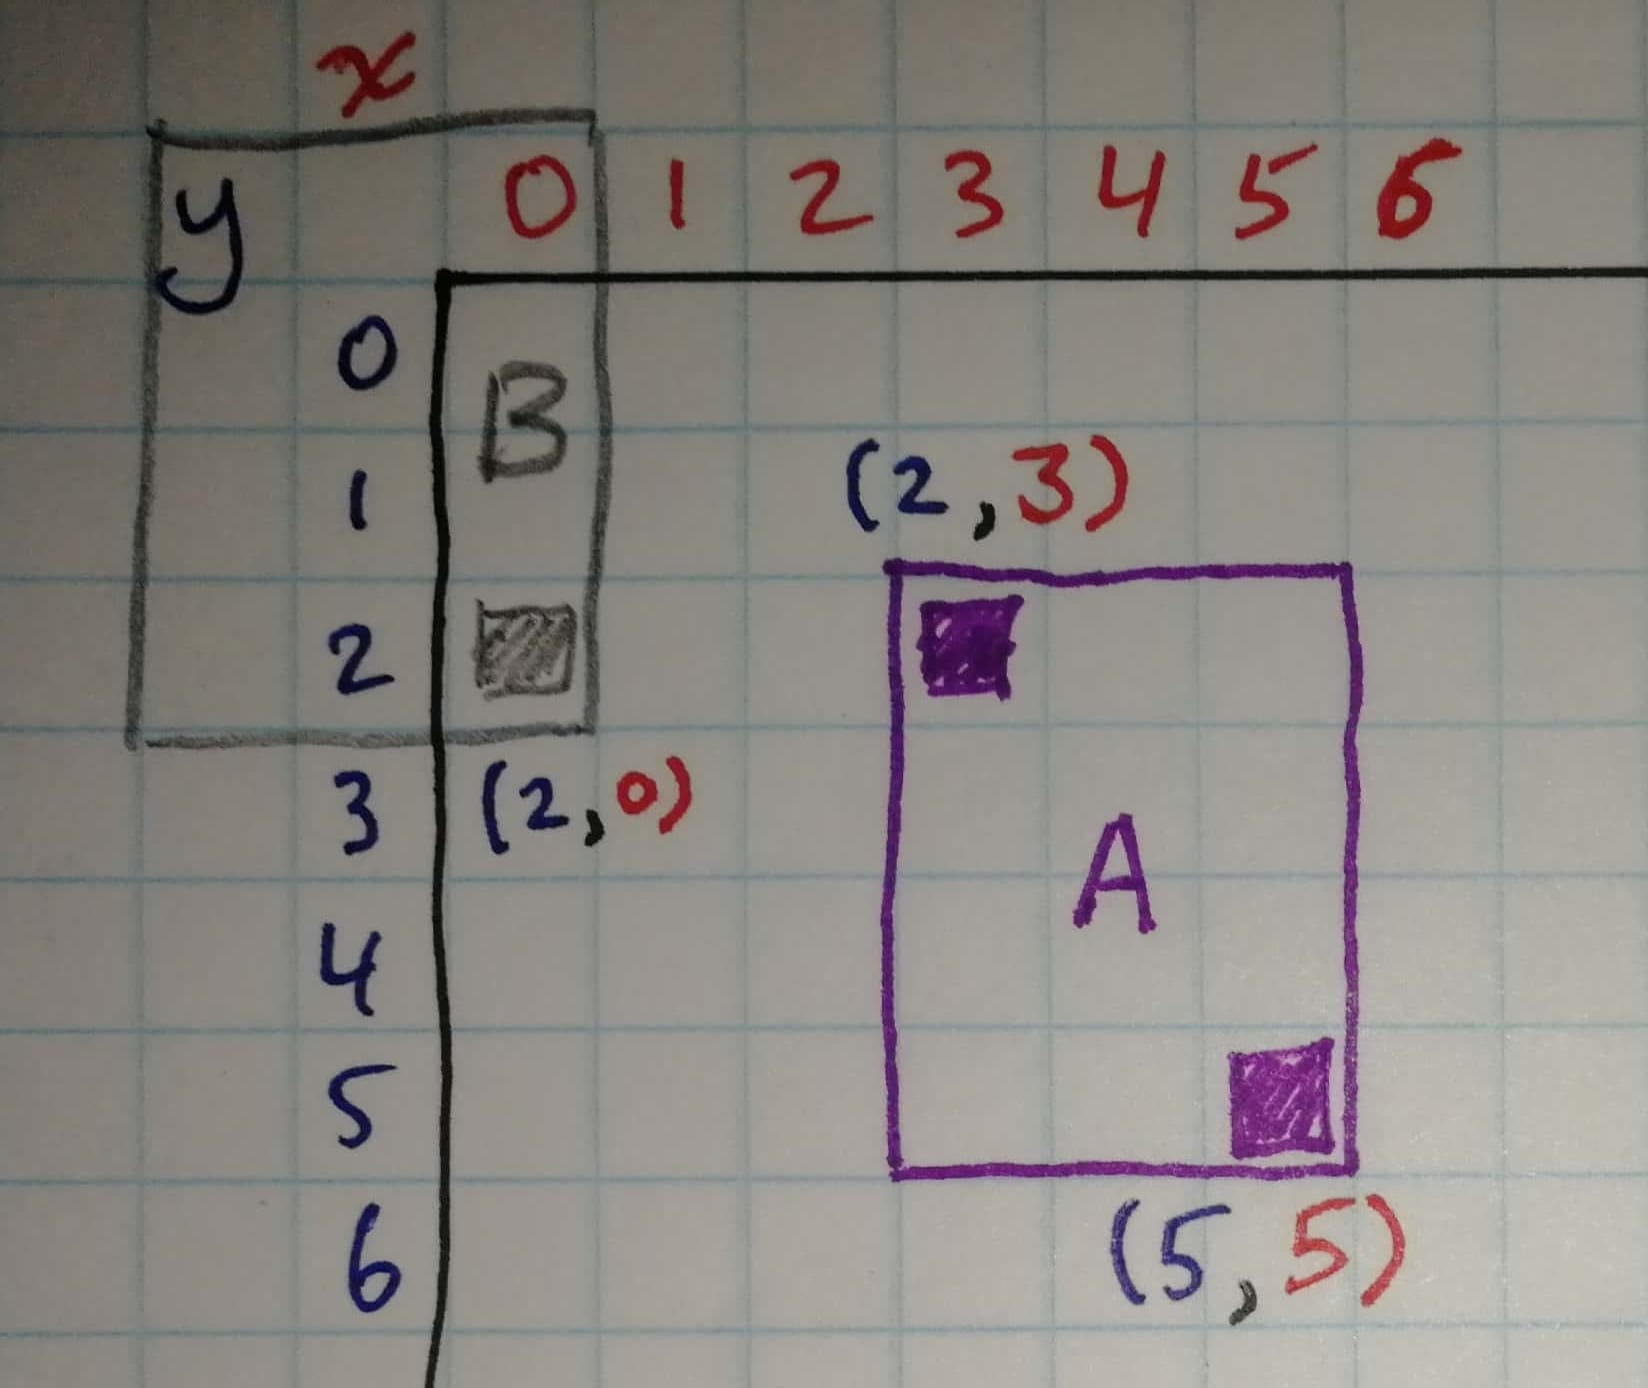
\includegraphics[width=0.5\linewidth]{Figures/old-line-buffer.jpg}

Window A (purple) is considered a valid output, but window B
(gray) is not a valid output by the old line buffer's rules.
\end{center}

The original line buffer could be parallelized by increasing the
number of pixels streamed in per clock cycle. Since (almost) each
input pixel corresponds to one output window's lower-right corner,
multiple output windows would be produced per cycle as well.

This plan seemed simple, but in practice such parallelized line
buffers were difficult to schedule. The main issue was that, with
multiple windows output per cycle, it's possible for some to be valid
and some to be invalid at the same time. Even with ready-valid timing,
this would require some
complicated lane-interleaving logic downstream from the line
buffer. Furthermore, even without paralellization, this line buffer
would be difficult to place in a synchronously-timed circuit
(i.e. non-ready-valid), since it produces an irregular output
pattern. The output is stalled each time the input ``passes over'' the
left margin of the image being streamed; for example, a line buffer
with a 4-pixel wide window would produce no valid output whenever
one of the first 3 pixels of a row is input.

To make scheduling managable, the original line buffer had several
divisibility requirements on its parameters. The most problematic
restriction was that the input pixels-per-clock\footnote{
  Strictly speaking, this parameter is horizontal pixels-per-clock.
  The old line buffer was also planned to support streaming multiple
  rows of pixels in per cycle, which I don't discuss here.
} had to divide both

\begin{enumerate}
\item Window width - 1
\item Image width - Window width + 1
\end{enumerate}

These restrictions were needed to prevent both valid and invalid
windows from being produced on the same cycle (Figure
\ref{old-lb-tiling.jpg}). In practice, few levels-of-parallelization
(besides 1) could satisfy both restrictions. Stencil sizes are
typically small, so ``Window width - 1'' already sets a low ceiling on
pixels-per-clock. ``Window width - 1'' more likely than not would be a
prime number, and, if ``Image width - Window width + 1'' did not share
that prime factor, the line buffer cannot be parallelized at all.

\begin{figure}
\centering
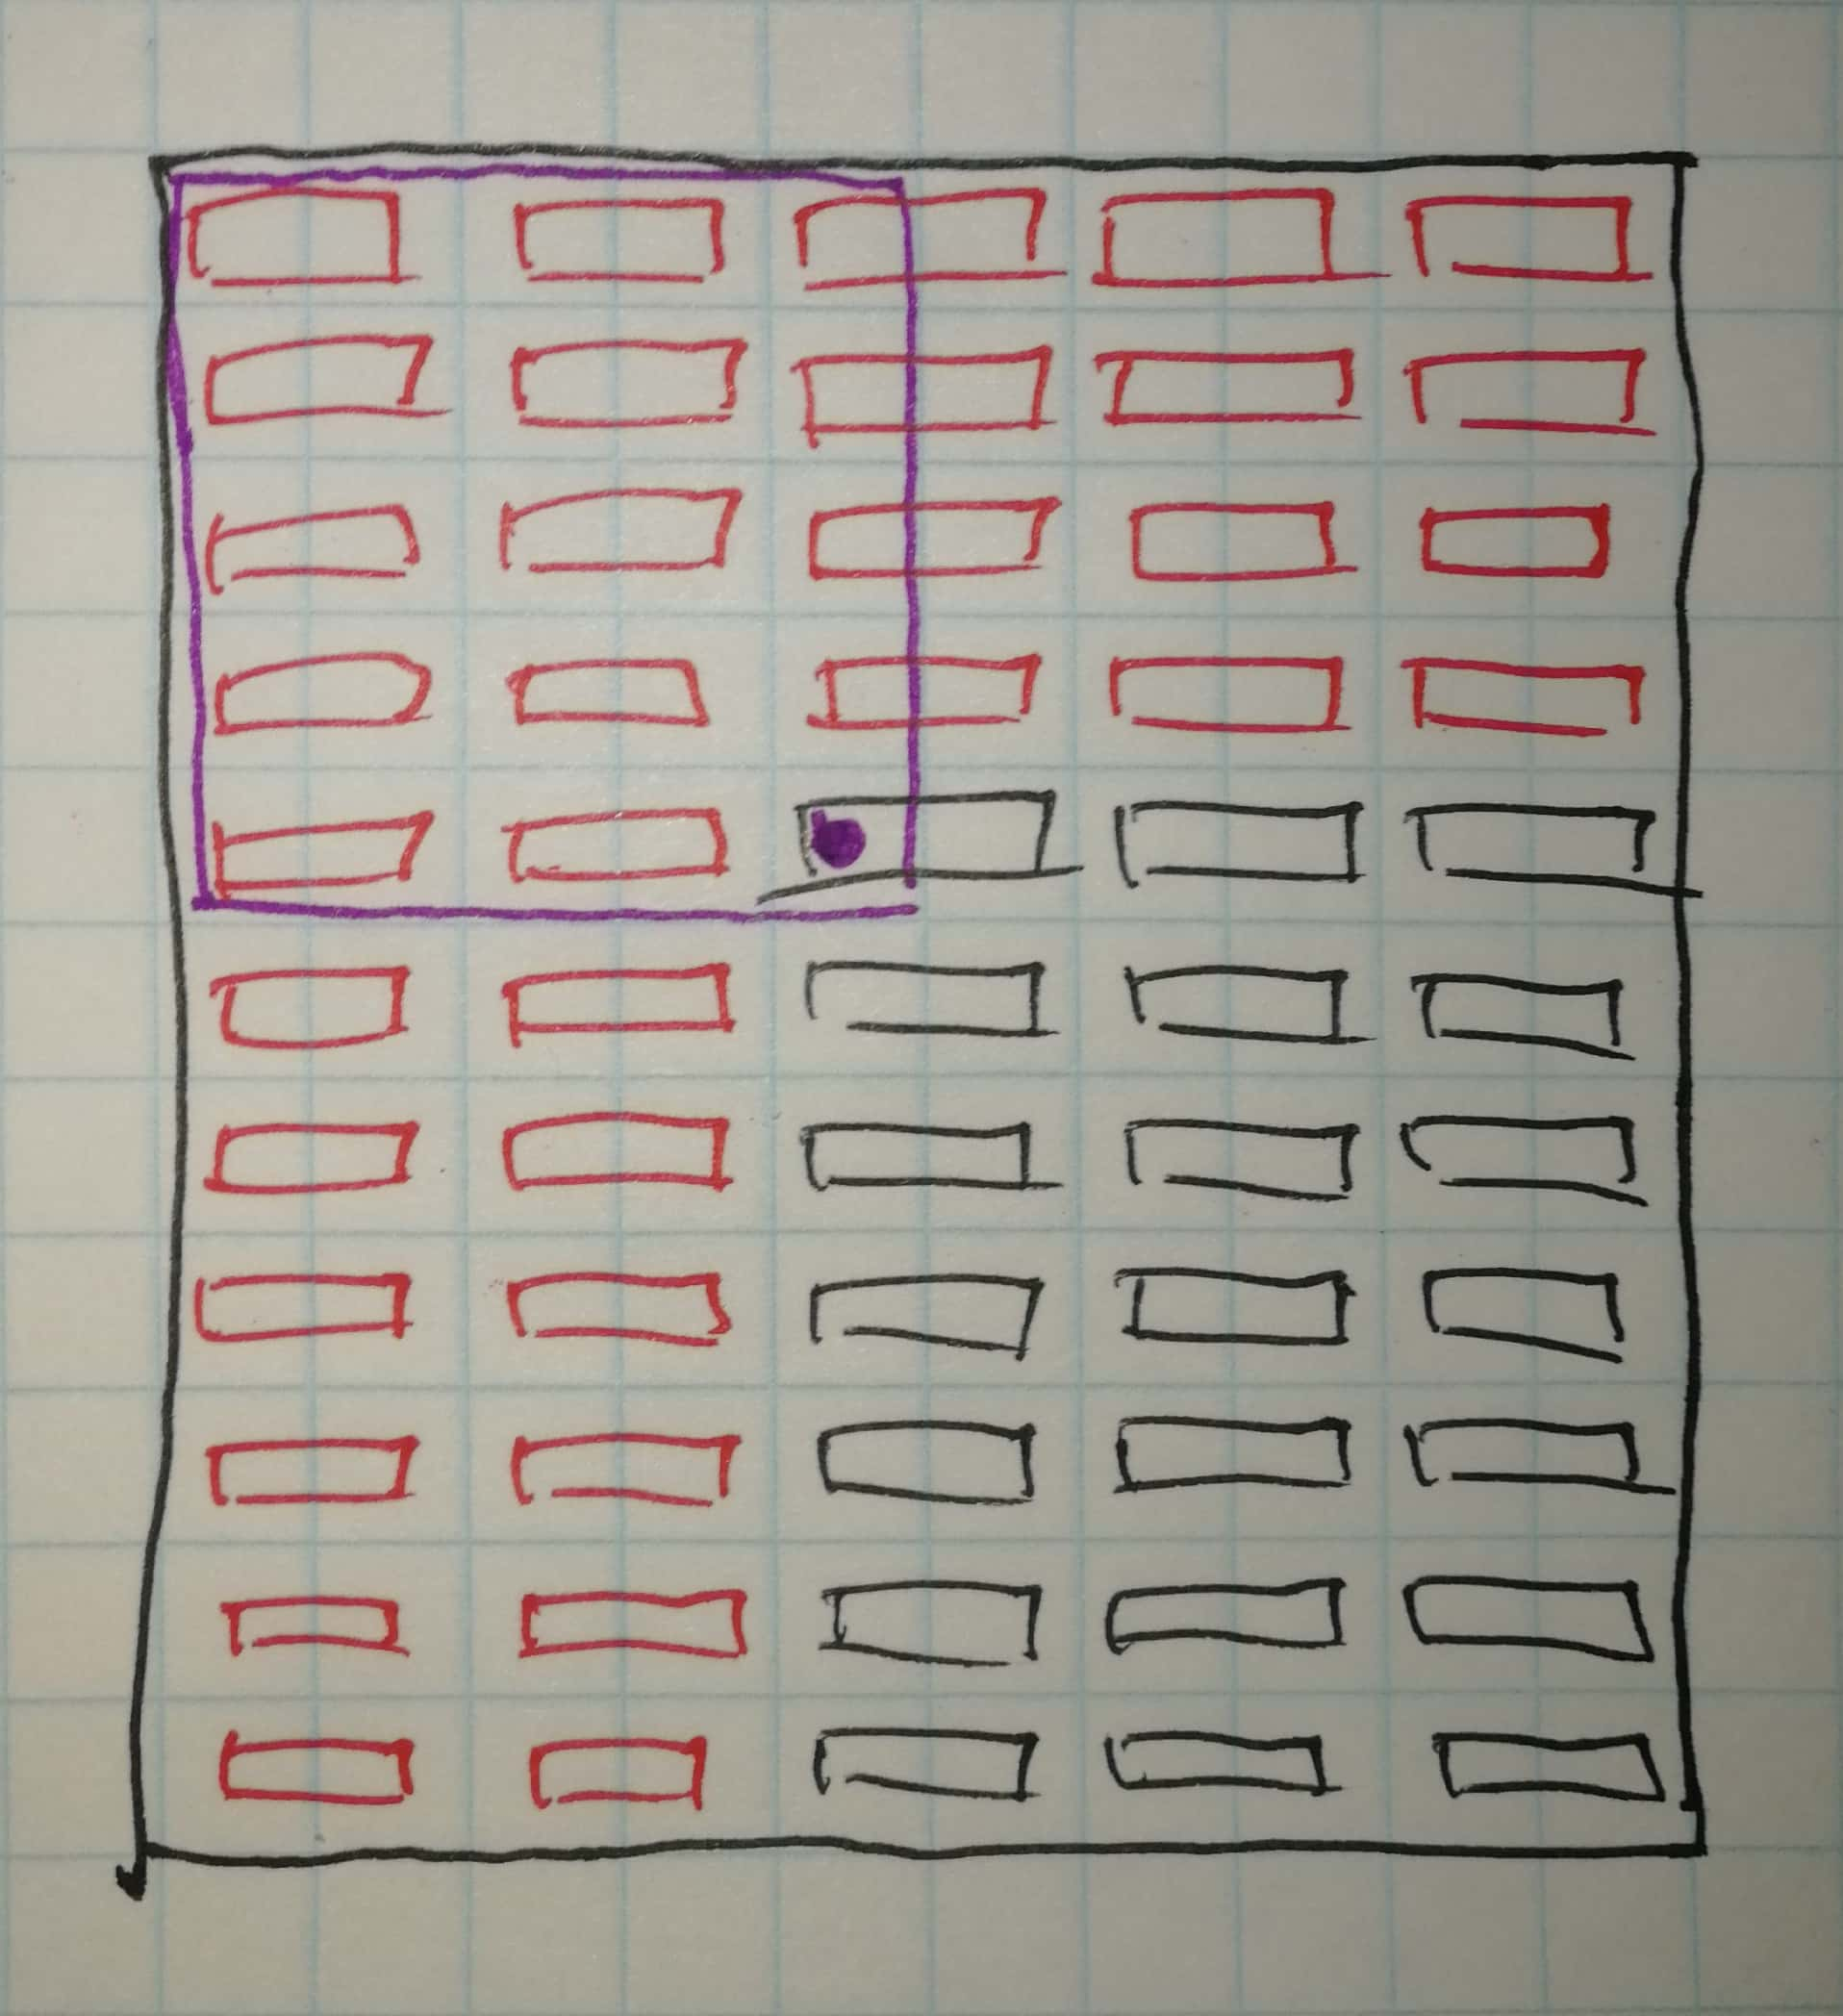
\includegraphics[width=0.5\linewidth]{Figures/old-lb-tiling.jpg}
\caption{Visualization of how input pixels tile an image. This line
buffer takes 2 pixels per clock, has a $5 \times 5$ window size,
and reads a $11 \times 10$ image. Red inputs produce no
valid output windows; black inputs produce only valid output windows
(under old line buffer rules).}
\label{old-lb-tiling.jpg}
\end{figure}

A further drawback of the original line buffer is that it did not
support an output ``stride''. Each output window is offset by 1 pixel
from its nearest vertical and horizontal neighbors. This prevents
mipmapping and pyramid-based image processing algorithms from being
expressed as Aetherling pipelines. (I think that Darkroom had a
similar issue).

The main problem with the old line buffer was that invalid ``garbage''
outputs could have two causes. It could be caused by out-of-bounds
pixel access, or it could be caused by scheduling (\texttt{ReduceOp}
is an example of an op that produces garbage due to scheduling. A
reduce that sums up 4-sequences of integers would produce garbage
outputs 3-out-of-4 cycles waiting for the full sequence to be made
available).

For the new line buffer that David Durst is implementing in hardware,
I proposed that invalid values should only result from scheduling, not
from out-of-bounds pixel access. If a window is scheduled to be
output, it should still be considered valid even if it contains
garbage out-of-bounds pixels. Global bounds analysis can be performed
at the end of an Aetherling pipeline to crop out the margins of the
final output image that were produced from garbage pixel values.  By
moving the responsibility of tracking out-of-bounds pixel access from
the individual line buffers to a single node at the end of the
circuit, we can get rid of the two most restrictive divisibility
requirements listed above.

I also proposed that the new line buffer should support output stride
(horizontal and vertical distance between windows) and origin (the
top-left corner of the initial output window). Vertical stride in
particular produces some scheduling difficulties that I proposed
(but did not implement in hardware) a solution to.

\subsection{New Line Buffer Parameters}

The new line buffer takes these parameters as pairs of $(height, width)$.

\begin{enumerate}
\item Input pixels per clock ($pxPerClk$)

This defines the ``shape'' of the 2D-array
input bus, and therefore how much more of the input image we see per
cycle.\footnote{For simplicity I talk as if the line buffer op is
fully utilized. If the line buffer is underutilized, then ``each cycle''
should be taken to mean ``each cycle when the line buffer is scheduled
to advance its state''.}

I originally proposed that the height of this parameter must be 1, but
the new line buffer may be extended to support streaming in multiple
rows per clock cycle. In this case, the height of this parameter
will be greater than 1, and the parameter's width must match the
image width.

\item Output window size ($window$)

\item Image size ($image$)

\item Output stride ($stride$)

The vertical and horizontal distance between the
upper-left corners of adjacent output windows.

\item Output origin ($origin$)

The upper-left coordinate of the initial output
window (itself the upper-left most window).
\end{enumerate}

The line buffer also takes a type parameter (e.g. it could be
parameterized with \texttt{tInts[3]} to process RGB pixels), and
there's talk of supporting a boundary condition parameter: I proposed
that the line buffer simply emit some garbage when it's scheduled to
output a window that overhangs the image boundaries, but it may be
useful to provide the line buffer with well-defined behavior when it
conceputally accesses an out-of-bounds pixel (something akin to
OpenGL's \texttt{GL\_TEXTURE\_WRAP} parameter).

\subsection{Input-Output Format}

The input is a 2D-array of pixels, with height and width given by the
pixels-per-clock parameter. Pixels are stored and streamed in reading
order: left-to-right, then top-to-bottom. (If the width of the input
array equals the width of the image, then the image is streamed-in one
(or more) row at a time, top-to-bottom).

Example: For a 9-pixel wide image and a $(1,3)$ pixels-per-clock
parameter, the first 4 cycles will see these pixels as input:

\begin{center}
\begin{tabular}{c|r r r}
cycle & input[0][0] & input[0][1] & input[0][2] \\
\hline
0 & (0,0) & (0,1) & (0,2) \\
1 & (0,3) & (0,4) & (0,5) \\
2 & (0,6) & (0,7) & (0,8) \\
\hline
3 & (1,0) & (1,1) & (1,2)
\end{tabular}
\end{center}

The output is a 3D-array of pixels: the inner 2 dimensions correspond
to the height and width of a window, and the outer dimension is for
parallelism (multiple output windows packed together, left-to-right).

For each image streamed in, the line buffer should produce
\begin{equation}
\frac{image_y}{stride_y}
\end{equation}
rows of valid output windows, each of which consists of
\begin{equation}
\frac{image_x}{stride_x}
\end{equation}
valid output windows.

\begin{table}
\centering
\begin{tabular}{| c c | c c | c c |}
\hline
X & X & O & O & X & X \\
\hline
O & O & X & X & O & O \\
\hline
X & X & O & O & X & X \\
\hline
O & O & X & X & O & O \\
\hline
\end{tabular}

\caption{
Visualization of how a line buffer's $4 \times 6$ image would be
broken down into $1 \times 2$ windows, with stride $1 \times 2$. (X
and O used to represent window regions). $\frac{4}{1} = 4$, so there
are 4 rows of output windows. $\frac{6}{2} = 3$, so there are 3 valid
output windows per row. If this line buffer takes 1 input pixel per
cycle, then every other cycle the line buffer's outputs are not
considered valid due to stride.}
\end{table}

Conceptually, stride is used for downsampling, so we expect that the
number of outputs should be divided by the stride. For example, if
we're using a line buffer to downsample a $2048\times 1024$ image by 2
in each direction with a Gaussian smoothing step, we would use a line
buffer with a $(2,2)$ stride, and expect $\frac{2048}{2}$ rows of
output windows, $\frac{1024}{2}$ windows per row, yielding a total of
$1024\times 512$ windows, each of which gets convolved to yield 1
pixel of the $1024 \times 512$ output image.

\begin{figure}[htb!]
  \centering
  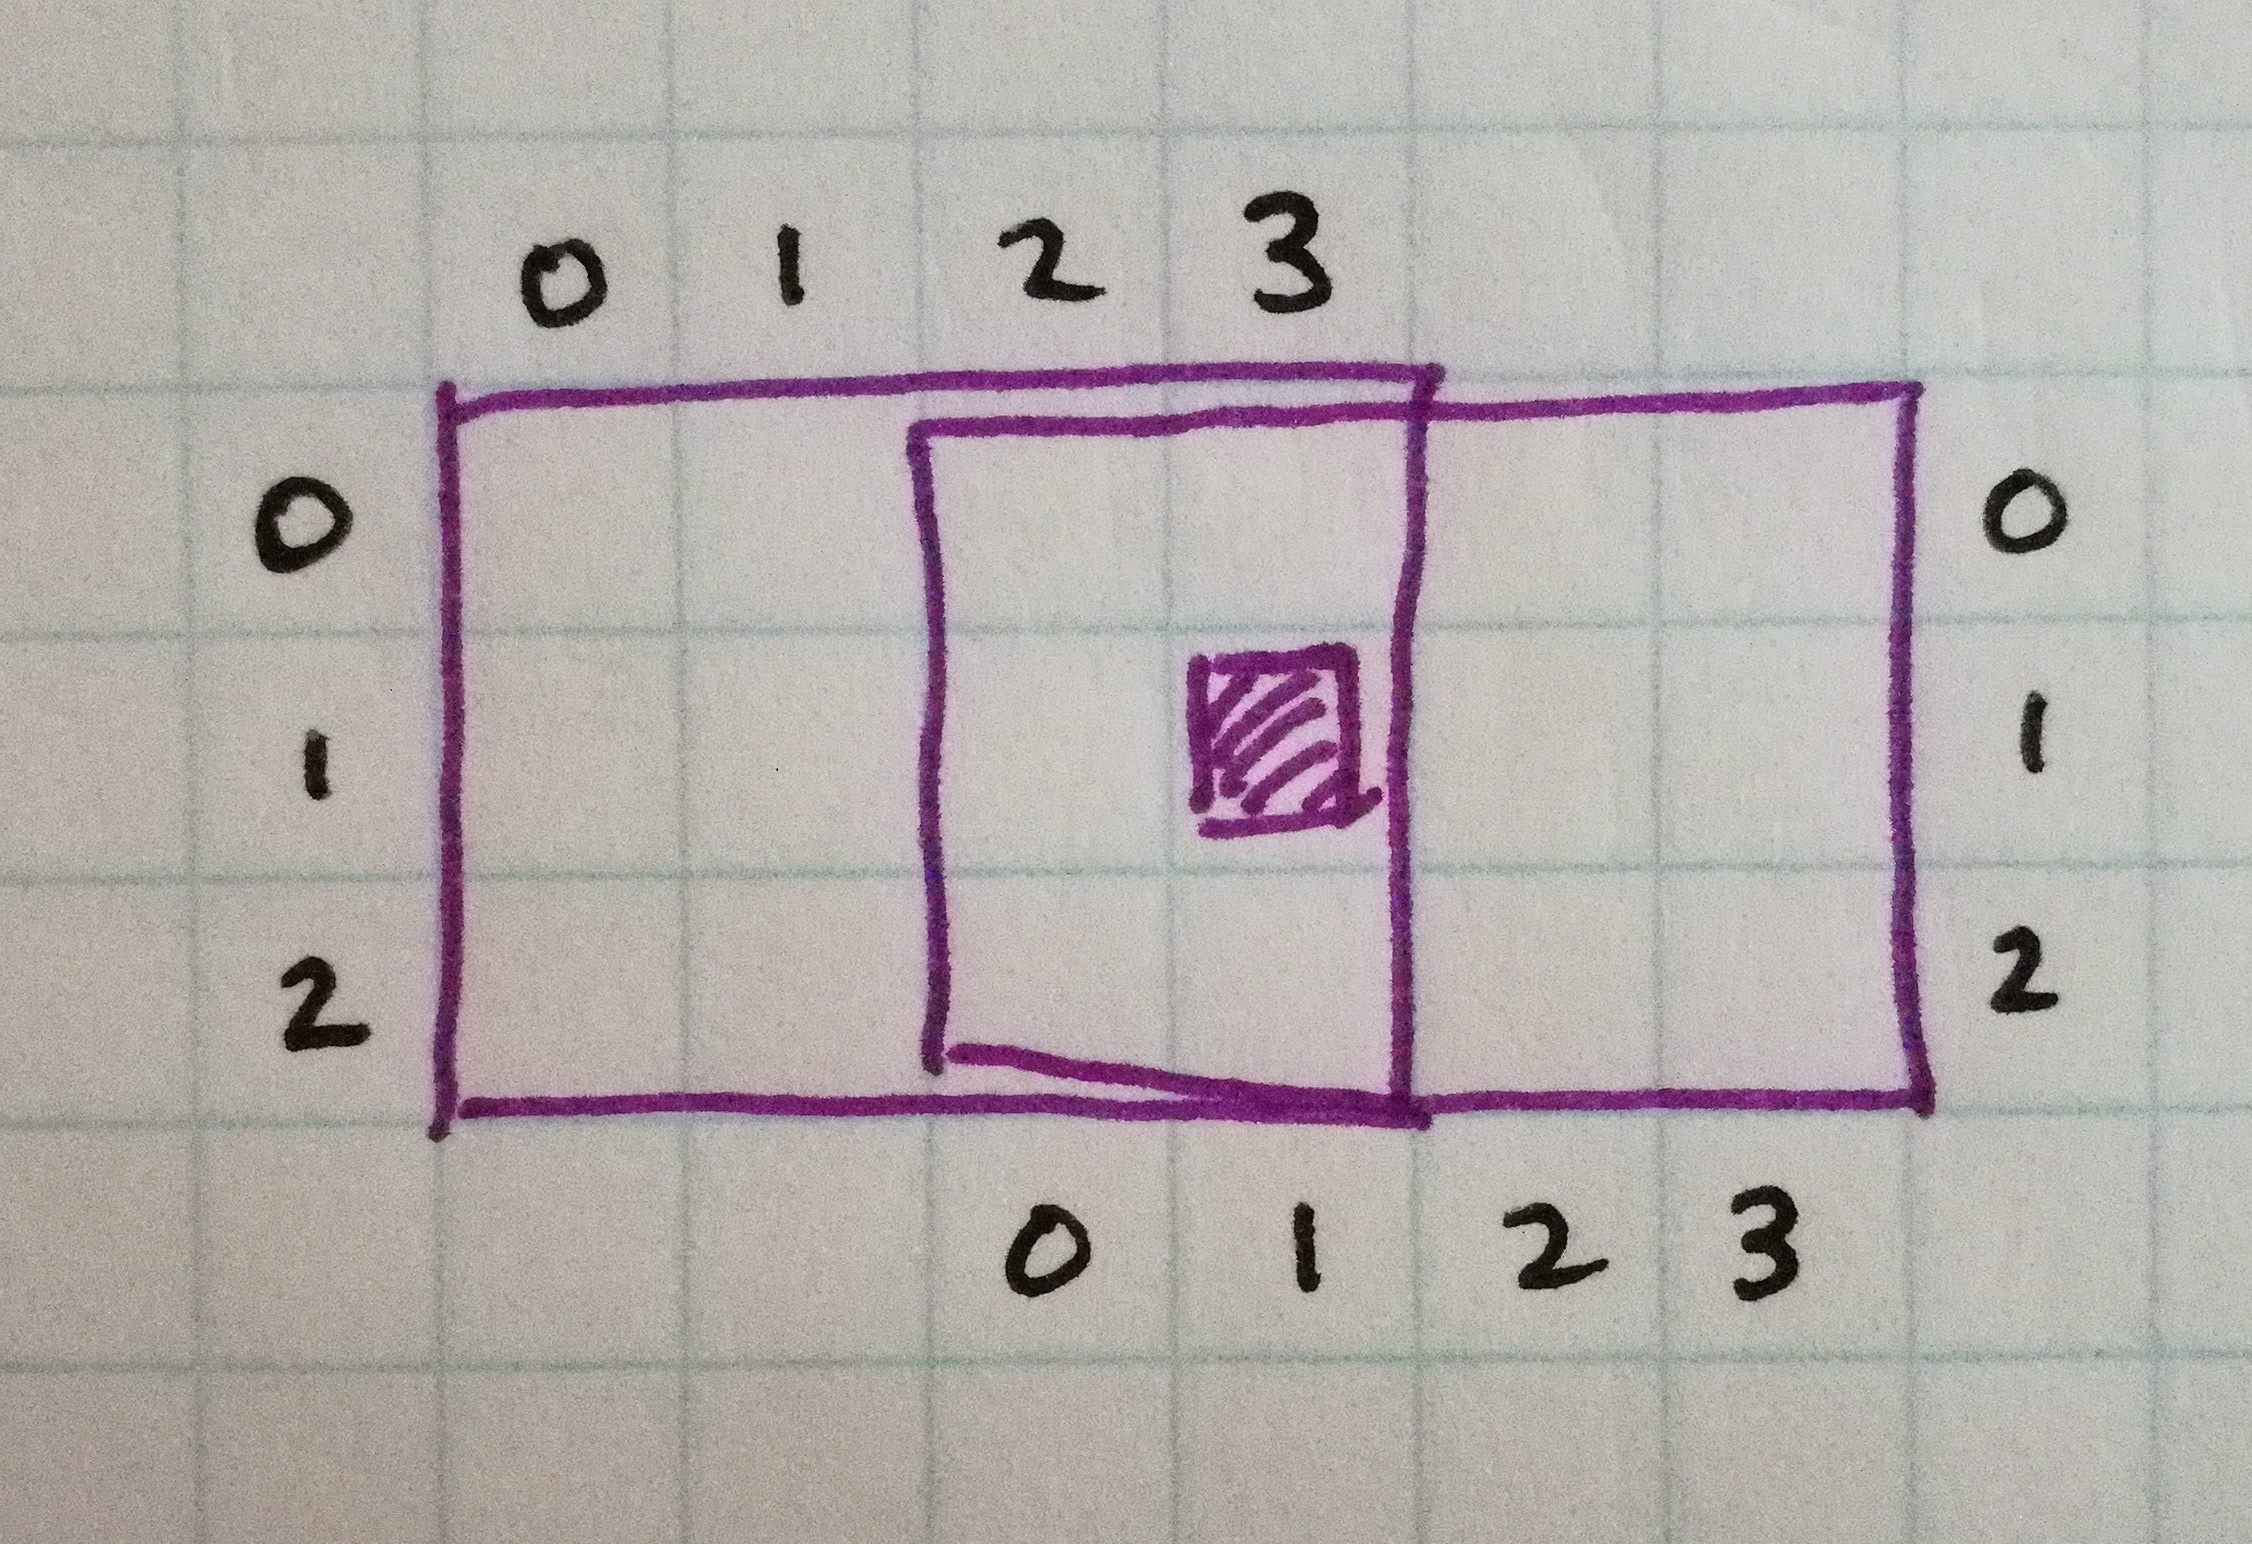
\includegraphics[width=0.6\linewidth]{Figures/lb-format.jpg}
  \caption{Figure representing one cycle's output of a line buffer
    with a $(3,4)$ output window size, an $x$-stride of 2, and 2
    output windows per clock. The output array dimensions are
    \texttt{[2,3,4]}, since there's a count of 2 output windows per
    cycle, and each window has a size of $(3,4)$. The highlighted
    pixel has coordinates \texttt{[0,1,3]} and \texttt{[1,1,1]},
    because it's at coordinate $(1,3)$ of the upper-left-most window
    (\texttt{O[0]}) and at coordinate $(1,1)$ of the \texttt{O[1]}
    window (the window 1 stride to the right of the \texttt{O[0]}
    window).}
  \label{4D_output}
\end{figure}

\subsection{Throughput and Schedule}

We define the ``window throughput'' as the average number of valid
output windows per cycle. I wanted to spread out the new line buffer's
outputs evenly through time to give the new line buffer a regular
output schedule. So, I calculate the throughput by dividing the total
number of output windows (per image) with the number of cycles it
takes the line buffer to stream in an entire image.

It takes
\begin{equation}
\frac{image_x image_y}{pxPerClk_x pxPerClk_y}
\end{equation}
cycles to stream in the entire image, and in that amount of time\footnote{
``in that \textit{amount} of time'', because there may be added latency.}
we must emit
\begin{equation}
\frac{image_x image_y}{stride_x stride_y}
\end{equation}
valid output windows. Dividing the two quantities, we have
\begin{equation}
    \text{Window throughput} = \frac
      {pxPerClk_x pxPerClk_y}{strides_x strides_y}
\end{equation}

The parallelism of the output array (i.e. its outermost dimension)
will be set to accomodate this many output windows per cycle (1 for
window throughput $\le1$).

If the window throughput is 1 or greater, then it should be an integer
$N$ (more on this later), and the line buffer is scheduled to start
with a certain number of latency cycles, where no valid outputs are
produced, then proceed to generate $N$ valid outputs every cycle.

If the window throughput is a fraction less than 1, then the line
buffer will generate at most 1 valid output per clock cycle.

These output windows are packed into the parallel output left-to-right,
then streamed left-to-right, row-by-row.

Especially for line buffers with $stride_y > 1$, evenly spreading out
the output windows through time breaks the relationship between a
given cycle's inputs and outputs. Unlike the old line buffer, where
each output window's lower-right pixel corresponds to a pixel input on
the same cycle, in the new line buffer there may be no clear
relationship between one clock cycle's outputs and inputs.

As an example, consider a line buffer with image size $(4,8)$,
stride $(2,2)$, and $pxPerClk$ $(1,8)$.

\begin{center}
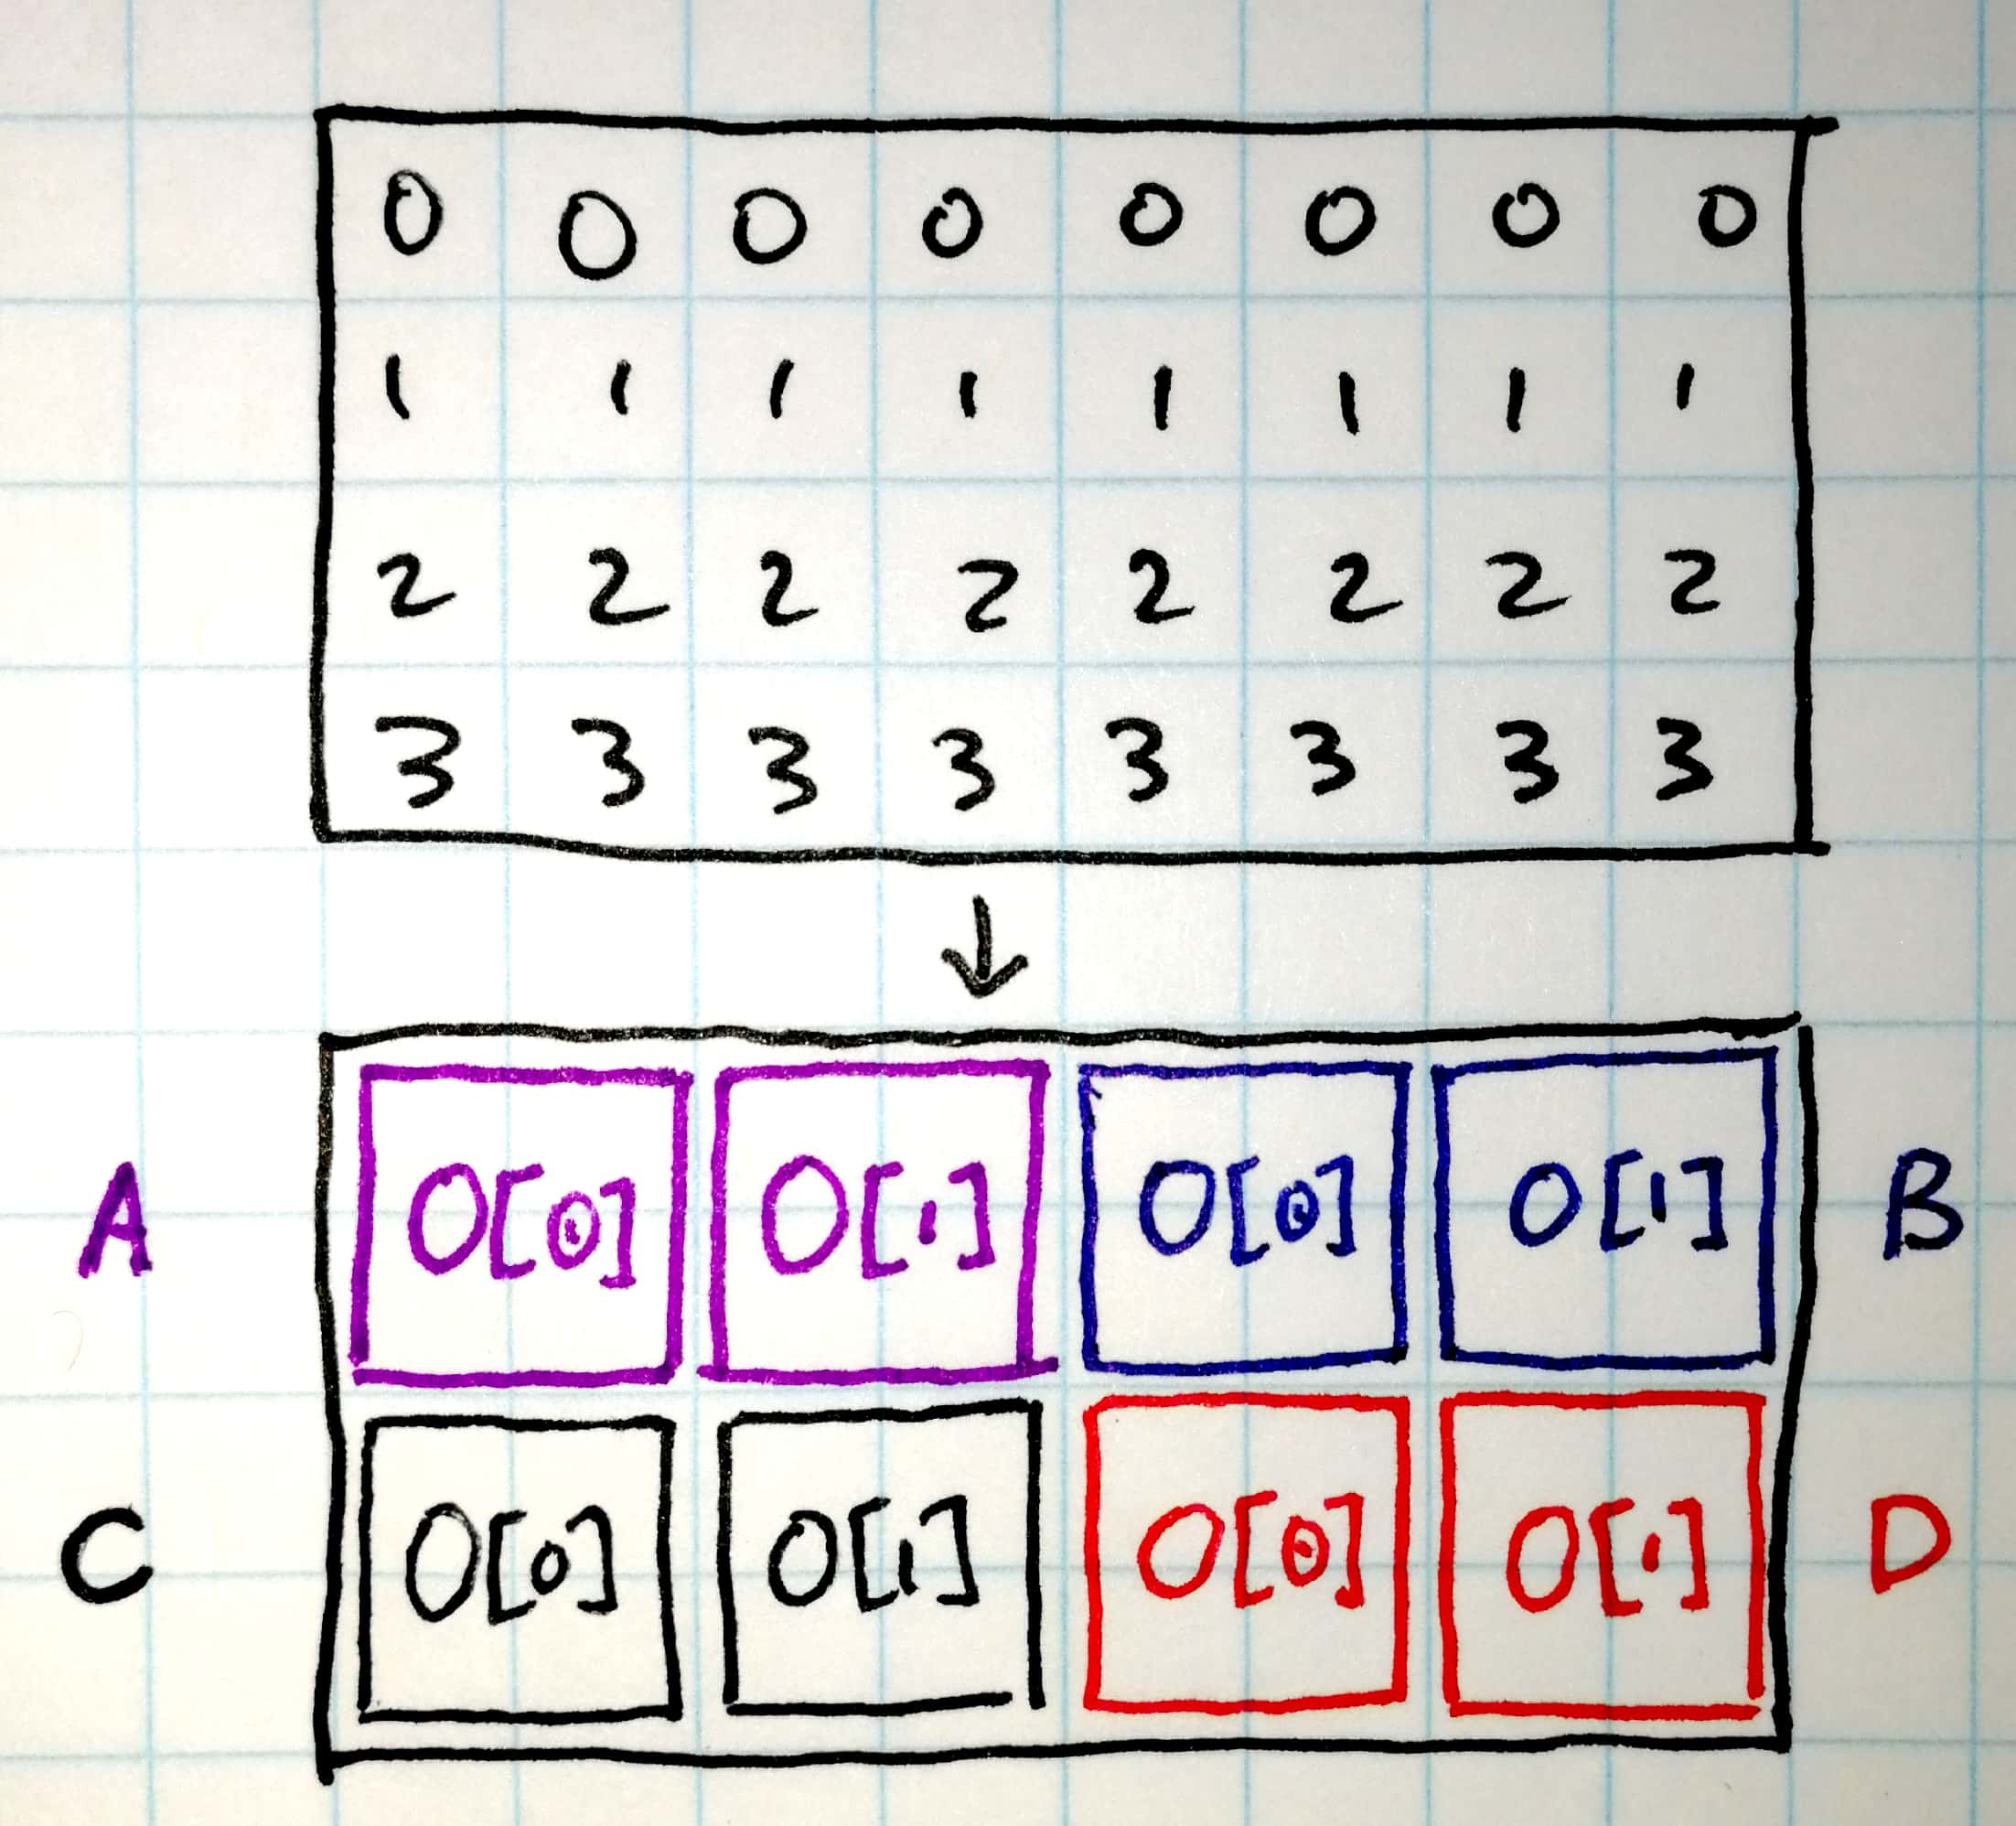
\includegraphics[width=0.6\linewidth]{Figures/lb-schedule.jpg}

Top: Image pixels labelled with the clock cycle they were input on.

Bottom: Output window schedule. Each color represents one cycle's output.
\end{center}

This line buffer reads in an entire row of the image per clock cycle,
and, dividing ($1\times 8$) by ($2\times 2$), we deduce that it should
emit 2 valid output windows per clock cycle. After waiting a certain
number of latency cycles (depends on implementation), the line buffer
should output the 2-window arrays A, B, C, and D over 4 clock cycles
with no pauses in between (unless the line buffer has been wrapped in
an underutilization op).

\subsection{Remaining Divisibility Requirements}

The remaining divisibility requirements are that
\begin{enumerate}
  \item The stride width (height) must divide the image width (height).
  \item The $pxPerClk$ width must divide the image width.
  \item The window throughput must be an integer or a reciprocal of an integer.
  \item If $pxPerClk$ height is not 1, then
  \begin{enumerate}
    \item $pxPerClk_x = image_x$.
    \item $pxPerClk_y$ must divide $image_y$.
    \item $pxPerClk_y$ must divide $stride_y$, or the other way around.
  \end{enumerate}
\end{enumerate}

The first two divisibility restrictions depend on the image
dimensions, so I expect them not to be too restrictive since typical
images have fairly composite dimensions. Furthermore, if multiple line
buffers are chained together with no downsampling ($stride = (1,1)$),
then all of them will have the same image size and will not impose
additional constraints on one another.

The $pxPerClk$ restrictions are justified by the difficulty of
implementing a line buffer that accepts portions of 2 different rows
in one clock cycle as input, or emits windows from two different rows
as output in one clock cycle.

The $stride$ restrictions have both conceptual and pragmatic
justifications. The conceptual justification is that stride is used
for downsampling, and we expect downsampling by a factor of $x$ should
scale the number of output samples (windows) by exactly $x^{-1}$ --
impossible if the image dimension is not itself a multiple of $x$.

The pragmatic justification is that scheduling becomes difficult
without this stride assumption. The window throughput calculations
were dependent on the total number of output windows being exactly
\begin{equation}
\frac{image_x image_y}{stride_x stride_y}
\end{equation}
This cannot happen if the strides do not divide the image
dimensions.\footnote{ In case this sounds more-or-less the same as the
  conceptual reason, the low-level justification is that, to keep the
  internal buffer size bounded, we need the number of input pixels per
  clock to match, on average, with the number of ``new'' output pixels
  per clock (``new'' in the sense that this pixel was not output as
  part of an earlier output window). It turns out that the average
  number of new pixels per window is equal to $stride_x stride_y$,
  leading to the constraint
  
  $pxPerClk_x pxPerClk_y = (\text{Window Throughput})stride_x stride_y$
  
  (rearrange to get the original Window Throughput calculation).  The
  issue is that this averaging doesn't work if the strides do not
  divide their respective image dimensions; the left margin's windows
  will have a greater-than-average number of new pixels, which will
  only be balanced out by the right margin's windows having a
  lower-than-average number of new pixels if the strides divide image
  dimensions.  See figure \ref{footnote-rambling.jpg} for
  visualization.  }

\begin{figure}[bth!]
  \centering
  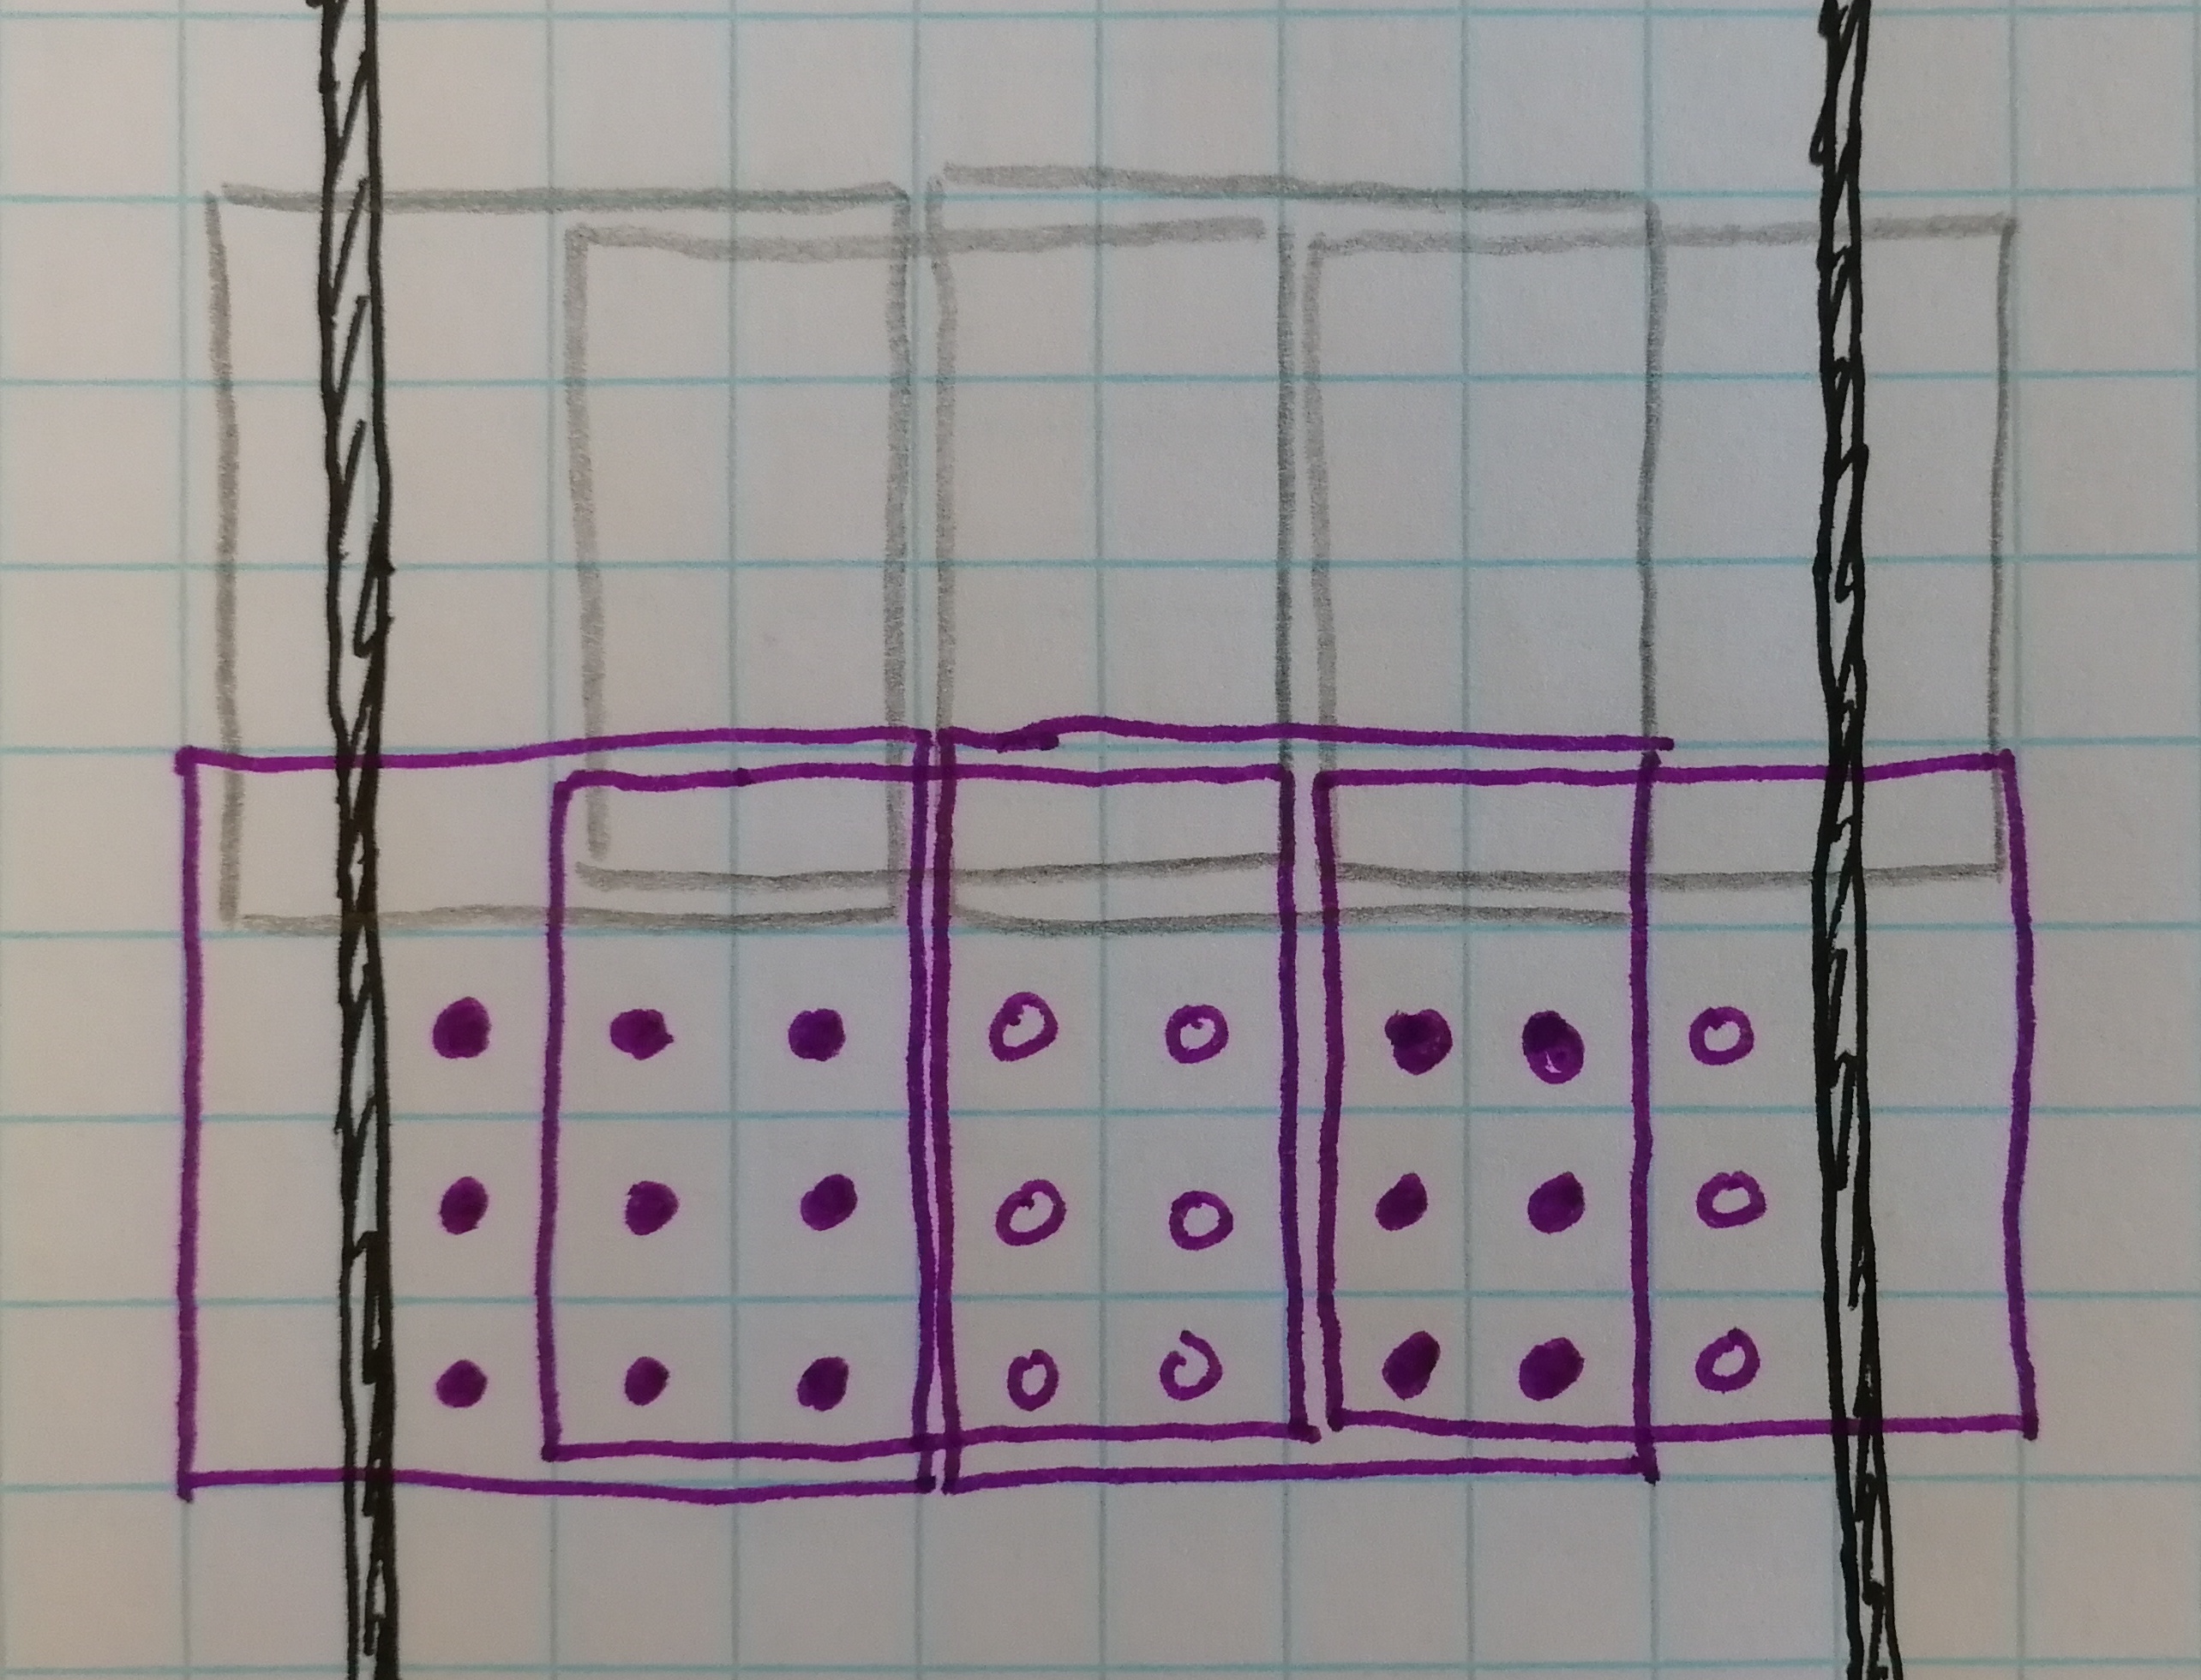
\includegraphics[width=0.6\linewidth]{Figures/footnote-rambling.jpg}
  \caption{Footnote example with image width 8, output window size
    $(4,4)$ and strides $(3,2)$. There are 4 windows per row of
    windows since image width 8 divided by $stride_x$ 2 is 4. Notice
    that the left-most window includes 9 new pixels and the right-most
    3, but on average each window requires emitting 6 new pixels,
    which matches the product of $stride_x$ and $stride_y$.}
  \label{footnote-rambling.jpg}
\end{figure}

The window throughput restriction is a bit more punishing, although
not as punishing as the old line buffer's divisibility restrictions.
This restriction was also motivated by scheduling concerns. It's not
clear how to schedule a line buffer that produces a fractional number
of valid output windows per cycle (with window throughput $>1$), and,
at the time I made my line buffer proposal, if window throughput were
less than 1, it also wasn't clear how to schedule line buffers with
window throughput not of the form $\frac{1}{N}$, $N:$integer. My phase
proposal might make it feasible to lift the window throughput
restrictions when window throughput is below 1.

\subsection{Chain of Line Buffers Example}

Consider a pipeline made up of two line buffers with combinational
stencil logic inserted between ($3 \times 3$ stencil) and after ($3
\times 5$) the line buffers. The two line buffers have
parameters\footnote{ Errata: It turns out that the upstream line
  buffer's latency is impossibly low -- the bottom-right pixel of the
  rightmost window each cycle has to travel back in time by 1 cycle.}
\begin{center}
\begin{tabular}{r|c c c c c c}
& $pxPerClk$ & $window$ & $image$ & $stride$ & $origin$ &
\texttt{sequentialLatency}
\\
Upstream line buffer & (1,4) & (3,3) & (6,12) & (1,1) & (-1,-1) & 3
\\
Downstream line buffer & (1,4) & (3,5) & (6,12) & (1,2) & (-1,-2) & 4
\end{tabular}
\end{center}

\begin{center}
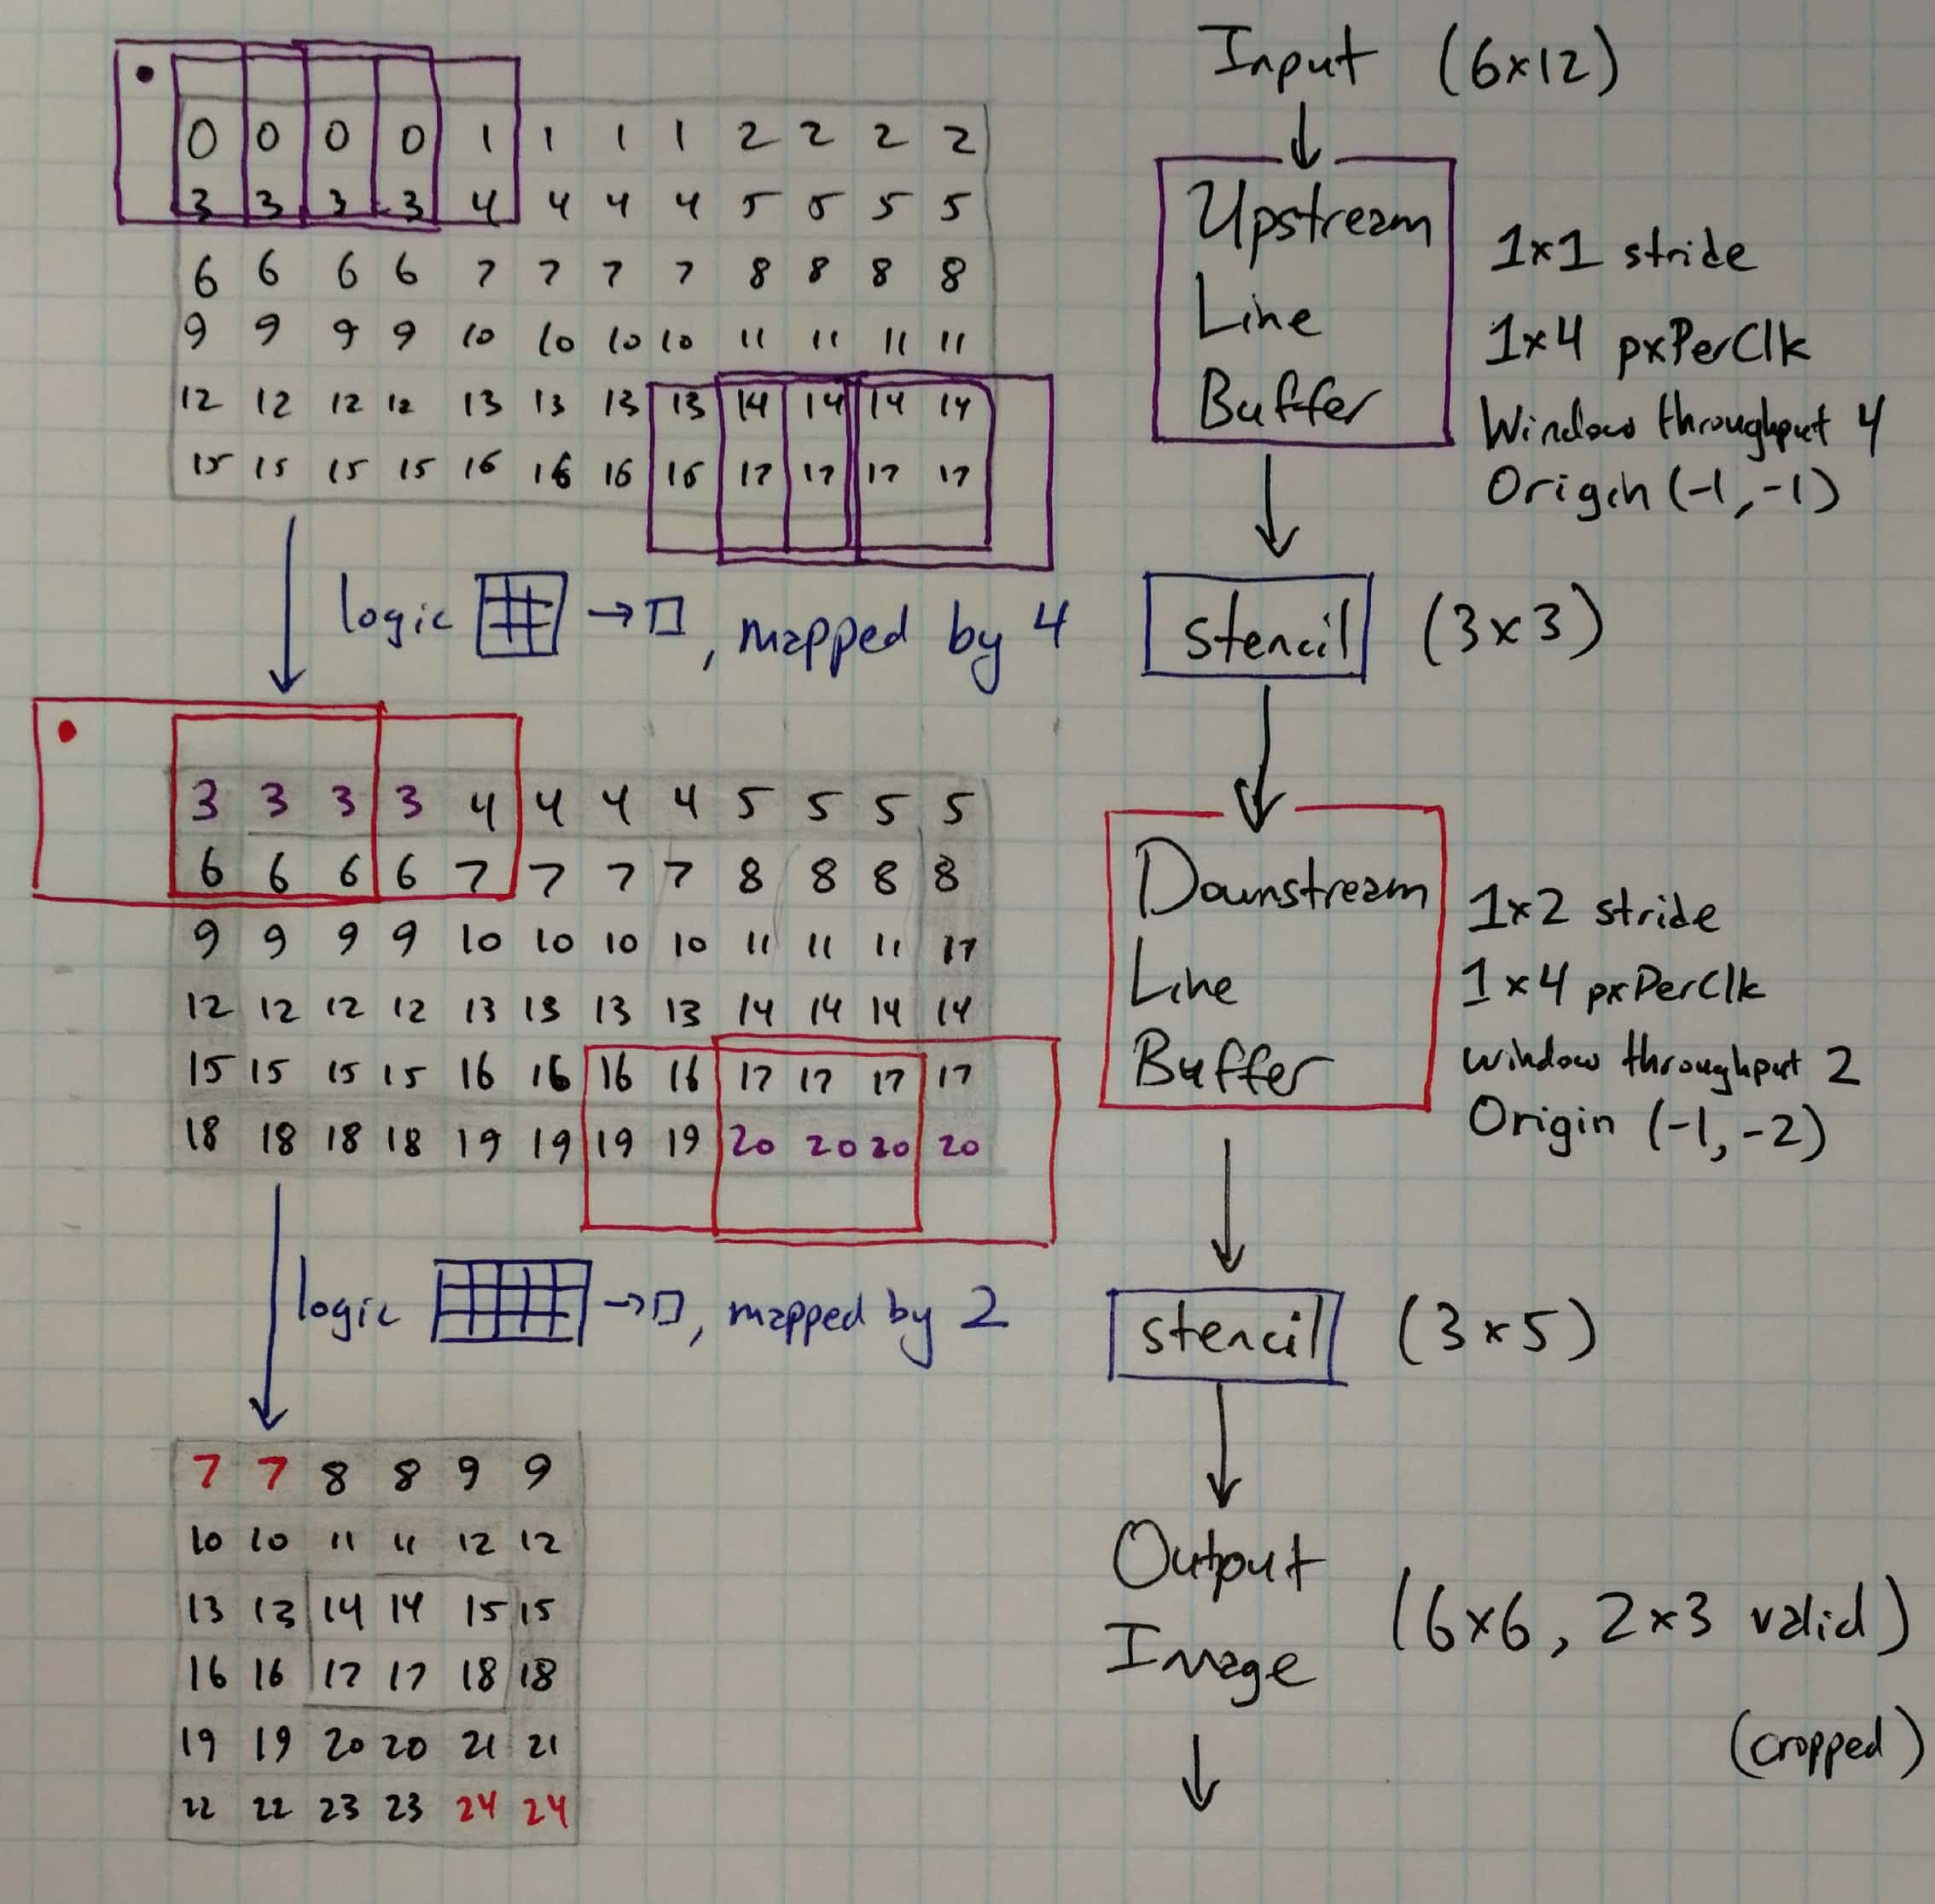
\includegraphics[width=1.0\linewidth]{Figures/lb-chain.jpg}
\end{center}

For the upstream line buffer, we have that
\begin{equation}
\text{Window throughput} =
\frac{pxPerClk_x pxPerClk_y}{stride_x stride_y} = 4
\end{equation}

So, there are 4 output windows per cycle (the initial and final batch
of windows are highlighted in purple), and, since both strides are 1,
the input and output images have the same size -- height 6, width
12. The $0^{th}$ output window of the initial valid output cycle
consists of the 9 pixels from (1,1) to the origin (-1,-1); this window
is still considered a valid output even though 5 of its pixels are
garbage values.

The stencil logic connecting the two line buffers must be mapped by 4,
since the upstream buffer produces 4 output windows per clock cycle.
Each pixel is labelled with the clock cycle that it is input to the
line buffer, and pixels whose values are based on windows with garbage
pixels are shaded in gray.

The downstream line buffer has the same $pxPerClk$ but a different
stride -- (1,2). This halves the width of its output image
(now $6\times 6$), and halves its window throughput to 2. The stencil logic
downstream of this line buffer, which produces the final output image,
is only mapped by 2 then.

Based on my proposed schedule for such a pipeline, the output image
has size $6 \times 6$ (18 valid outputs of 2 pixels each). However,
at the end of the pipeline, we may change our definition of ``valid''
to exclude garbage pixel values. Using bounds analysis we can conclude
that the valid portion of the output image has size $2 \times 3$.

\section{Functional Simulator}

Note: \texttt{src/Core/Aetherling/Simulator/README.md} in the
\texttt{aetherlingHaskellIR} source tree is the main source of
documentation for the functional simulator.

The functional simulator (\texttt{simulateHighLevel} function) was the
first contribution I made to the Aetherling project. At the time, the
plan for timing Aetherling ops wasn't clear, and many of the ops were
not realized in hardware yet, so it seemed important to write a
high-level simulator that did not concern itself with precise hardware
details like timing.

The data type that the simulator operates on is a ``stream'' of
\texttt{ValueType}: this represents the values of a port's valid
outputs through time, with no timing details included. Input is passed
to a simulated op with multiple ports as a list of streams,
represented in Haskell as a 2D-list of \texttt{ValueType}, with the
outer dimension corresponding to ports and the inner dimension
corresponding to time.

As a simple example, consider simulating an adder:

\begin{verbatim}
inputs = [
    [V_Int 0, V_Int 2, V_Int 4],
    [V_Int 30, V_Int 20, V_Int 10]]
simulateHighLevel (addInts T_Int) inputs [] -- empty memory argument

outputs: ([V_Int 30, V_Int 22, V_Int 14], []) -- empty memory result
\end{verbatim}

(\texttt{V\_Int} constructs a \texttt{ValueType} representing a
simulated integer value).

Assuming the adder is timed to perform one add per cycle, this simulation
corresponds to an adder calculating
\begin{center}
\begin{tabular}{c|c c|c}
cycle & port 0 input & port 1 input & result\\
0 & 0 & 30 & 0 + 30 = 30 \\
1 & 2 & 20 & 2 + 20 = 22 \\
2 & 4 & 10 & 4 + 10 = 14
\end{tabular}
\end{center}
over 3 clock cycles.

The reason I chose the outer dimension of the input list to correspond to
port and the inner dimension correspond to time is that it's not possible
to represent inputs the other way without knowing details of the simulated
pipeline's timing.

Consider a pipeline with two input port. This pipeline reads a 4-sequence
of integers from port 0 and a single integer from port 1; sums up the
4-sequence, multiplies the single integer by 16, and outputs the
maximum of those two values. We can write this pipeline as

\begin{verbatim}
add4stream = arrayReshape [T_Int] [tInts [1]] |>>=| reduceOp 4 1 (addInts T_Int)
pipeline = (add4stream |&| underutil 4 (Shl 4)) |>>=| underutil 4 (maxInts T_Int)
\end{verbatim}

Simulate the pipeline with 2 input sequences using

\begin{verbatim}
inputs =
    [ -- port 0 input
      [V_Int 1, V_Int 2, V_Int 3, V_Int 4, V_Int 5, V_Int 6, V_Int 7, V_Int 8],
      -- port 1 input
      [V_Int 0, V_Int 10] ]
simulateHighLevel pipeline inputs []
\end{verbatim}

The port output should be \texttt{[10, 160]}: each input sequence
results in a single output. The $0^{th}$ 4-sequence on port 0 is
\texttt{[1, 2, 3, 4]}, and the $0^{th}$ 1-sequence on port 1 is
\texttt{[0]}, so we expect output \texttt{[0]} to be
\begin{equation}
    \max(1+2+3+4, 0 \text{ shl } 4) = \max(10, 0) = 10
\end{equation}

Output number \texttt{[1]} should be based on the $1^{st}$ input
4- and 1- sequences on ports 0 and 1, so we expect to see
\begin{equation}
    \max(5+6+7+8, 10 \text{ shl } 4) = \max(26, 160) = 160
\end{equation}

The important point is that entry \texttt{[1]} of the port 1 input
(\texttt{...V\_Int 10]}) is automatically matched with 4-sequence
input number \texttt{[1]} on port 0,
\texttt{...V\_Int 5, V\_Int 6, V\_Int 7, V\_Int 8]}. This could
not have been done if the input 2D-list's dimensions were swapped
without knowing the precise timing of the circuit. In this case,
the timing will be for port 1's input to come in as the last
($3^{rd}$) input of port 0's 4-sequence comes in, so, if the simulator
were written with the input dimensions swapped (time outer, port
inner dimension), the input may look something like

\begin{verbatim}
-- port 0 (4-sequence)
--   V
--   V    port 1 (1-sequence), X denotes invalid input
--   V      V
[ -- V      V
  [V_Int 1, X],       -- cycle 0 input
  [V_Int 2, X],       -- cycle 1 input
  [V_Int 3, X],       -- cycle 2 input
  [V_Int 4, V_Int 0], -- cycle 3 input
  [V_Int 5, X],       -- cycle 4 input
  [V_Int 6, X],       -- cycle 5 input
  [V_Int 7, X],       -- cycle 6 input
  [V_Int 8, V_Int 10] -- cycle 7 input
]
\end{verbatim}

In general though, at the time the simulator was written, it would not
have been possible to deduce exact timing in all cases.

\subsection{Implementation Notes}

Aetherling (at the time of writing) defines two memory ops:
\texttt{MemRead} and \texttt{MemWrite}. Unlike port inputs and
outputs, which only appear at the beginning and end of a pipeline,
memory inputs and outputs could appear at any stage of an Aetherling
pipeline. Distributing \texttt{MemRead} values and collecting
\texttt{MemWrite} values properly was difficult to implement in the
simulator.

The first problem is that the individual \texttt{MemRead} and
\texttt{MemWrite} ops have no names, making it hard to even specify
the inputs and outputs. The solution I came up with for the time being
is to number each \texttt{MemRead} and \texttt{MemWrite} based on the
order they would be visited by a depth-first search of an Aetherling
AST.\footnote{Strictly speaking, the memory ops are numbered based on
  the order they would be visited by a DFS of an Aetherling AST
  transformed by duplicating ops by the number of times they actually
  appear in a physical circuit. Aetherling defines ops like
  \texttt{MapOp n} that have one child node that represents \texttt{n}
  copies of the actual op. If that op contains memory ops, each needs
  to be numbered separately.}

Internally, the simulator works by specializing the
\texttt{simhl}\footnote{ \textit{sim}ulate \textit{h}igh
  \textit{l}evel} function for each op offered by Aetherling.
The \texttt{simhl} function gets passed

\begin{enumerate}
\item A list of port input streams (in 2D-format as in \texttt{simulateHighLevel}).
\item A \texttt{SimhlState} instance.
\end{enumerate}

and returns

\begin{enumerate}
\item A list of port output streams (2D-list format)
\item The input \texttt{SimhlState}, modified by the op and its children.
\end{enumerate}

The main purpose of of the \texttt{SimhlState} type is to distribute
and collect memory inputs/outputs. It holds two lists of ``memory
tapes'' (themselves lists of \texttt{ValueType}, just like simulator
port inputs), one for memory inputs and one for outputs. A tape is
popped from the input list whenever \texttt{SimhlState} is passed to a
\texttt{simhl MemRead} call, with the popped tape used as the
\texttt{MemRead}'s simulated output stream. Similarly, a tape is appended to
the output list by \texttt{simhl MemWrite}.

To support the DFS-based order the user is expected to pass memory
inputs in, the user's memory arguments are pasted into the
\texttt{SimhlState} directly, then, each op's \texttt{simhl}
implementation is expected to thread the \texttt{SimhlState}
through all of its child op's \texttt{simhl} calls. (Here,
thread means to pass the \texttt{SimhlState} as an argument to
\texttt{simhl} and use the returned \texttt{SimhlState} instead
of the original \texttt{SimhlState} going forward).

Example: If the \texttt{simhl} call for \texttt{ComposePar [a, b]}
receives \texttt{state} as its \texttt{SimhlState} argument, then that
\texttt{state} should be passed to the \texttt{simhl a} call (along
with port inputs), yielding \texttt{SimhlState state'}. This
\texttt{state'} is passed to \texttt{simhl b}, resulting in
\texttt{state''}, which should be the final \texttt{SimhlState} value
returned by \texttt{simhl \$ ComposePar [a, b]}. \texttt{simhl a} and
\texttt{simhl b} are themselves expected to thread \texttt{SimhlState}
through any child ops they have, so, the final \texttt{state''} output
has been threaded through the entire AST anchored at
\texttt{ComposePar [a, b]} in DFS order.

\section{Demonstration Apps}

%% Talk about how writing apps led to realizations of what new line buffer needs?

\section{Simplifying Ops \& Helper Functions}

Previously, many Aetherling arithmetic ops (e.g. \texttt{Add}) took a
type parameter, which could be an array type. This meant that there
were multiple ways to express the same operation. For example, a bit
xor could be expressed as \texttt{XOr T\_Bit} or \texttt{Add T\_Bit},
and elementwise addition of two 4-arrays-of-int could be expressed as
\texttt{Add \$ T\_Array 4 T\_Int} (4-array type parameter) or as a
\texttt{MapOp 4} over a scalar \texttt{Add T\_Int}.

Since each op of the Aetherling Haskell IR will eventually need to be
implemented in hardware, it would be best to minimize unneeded
functionality as much as possible. I eliminated the type parameter
from arithmetic ops, splitting the op into two ops if bit and integer
versions are both needed (e.g. \texttt{And} for boolean $and$;
\texttt{AndInt} for bitwise $and$).

Since this change makes vectorized arithmetic harder to express
directly, I wrote some helper functions for expressing array types and
array operations. For example, a $16\times 16$ matrix of integers can
be expressed as \texttt{tInts[16,16]}, and an op performing
elementwise addition of two matrices can be expressed as
\texttt{addInts \$ tInts[16,16]}. Internally, the IR represents
vectorized ops as scalar ops wrapped by \texttt{MapOp}.
In this example, \texttt{addInts} will return

\texttt{MapOp 16 (MapOp 16 Add)}

The helper functions also serve the purpose of checking for invalid
parameters. For example, the function for creating a line buffer
op\footnote{Temporarily named \texttt{manifestoLineBuffer}.} checks that the
divisibility requirements are satisfied, and the \texttt{arrayReshape}
function, which creates an \texttt{ArrayReshape} op that reinterprets
inputs as a different type, checks that there's a reasonable mapping
between input and output types.\footnote{
Examples: \texttt{arrayReshape [tBits[2]] [T\_Bit, T\_Bit]} (conversion of
2-array-of-bit to two separate bits) is valid, while
\texttt{arrayReshape [tBits[3]] [T\_Bit]} is not since the input has
more bits than the output.}

\section{ReadyValid Op}

\section{ComposePar Retiming}

The \texttt{ComposePar} node of an Aetherling AST takes a list of
child ops, and represents placing that list of ops in parallel in
hardware. It's important that all these ops have the same latency when
the hardware is realized, so I wrote a retiming pass that visits each
\texttt{ComposePar} of an AST, and adds register ops as needed to make
all child ops of \texttt{ComposePar}s have matching latencies.

Solving the problem correctly is simple enough; the challenge was to
do it efficiently, with as few additional register bits as possible.

Before describing this solution, I should point out that we made one
compromise on the definition of an efficient solution. We decided
that, with few exceptions\footnote{Ops lacking either input or output
  ports (e.g. \texttt{MemWrite}, and ops with ready-valid interface)},
a \texttt{ComposePar}'s child ops should always have the same
latencies, even though it may be possible to have a correct pipeline
with some mismatched \texttt{ComposePar}s. See \footnote{Suppose
a, b, c, and d are all one input, one output port ops, a and d have 0
latency, b has 5 latency, and c has 10 latency. Consider the pipeline
\texttt{(a |\&| b) |>>=| (c |\&| d)}. To make both \texttt{ComposePar}'s
(\texttt{|\&|}) match, we would have to delay a with 5 registers
and d with 10 registers. However, c has no dependency on b and d has
no dependency on a, so we could have just delayed b by 5 cycles so
that the a,c and b,d paths both have 10 latency. We considered
this performance issue not to be too serious: we encourage users to
write pipelines as a \texttt{ComposePar} of \texttt{ComposeSeq}s if
possible. In this case, the functionally-identical pipeline would
be \texttt{(a |>>=| c) |\&| (b |>>=| d)}, which my retiming pass would
fix by adding just 5 register delays to \texttt{b |>>=| d}.
} for an example.

Another small thing to mention is that I replaced the \texttt{Delay}
op, which takes one child op to delay with registers, with a leaf
\texttt{Register} op. I did this because the \texttt{Delay} op either
\begin{enumerate}
\item Left ambiguous whether the registers were on the inputs or
  outputs of the wrapped op, or,
\item If one of those choices were defined as standard, the
  \texttt{Delay} op is not expressive enough to convey one
  possible delay choice -- either the choice of placing a delay
  at the very end, or at the very beginning, of a pipeline.
\end{enumerate}
The new \texttt{Register} op can be used by being composed in
sequence with the op to be delayed (using operator \texttt{|>>=|}).

The basic idea behind my recursive retiming pass is that, when it
operates on an Aetherling AST (or a subtree representing a portion of
the pipeline), it
\begin{enumerate}
\item Matches the latencies of all child ops of \texttt{ComposePar}
  found in the subtree, unless the child ops have ready-valid timing and
  the user elected to skip latency matching for such ops.

\item Increases the latency of the passed subtree by an
  \textit{additional} latency delta, beyond what is needed to just
  make all \texttt{ComposePar} children match.

\item Returns the cost (in register bits) of additionally delaying the
  portion of the pipeline passed by \textit{latency delta}.
\end{enumerate}
The motivation for \textit{latency delta} and the cost result comes
from the case of \texttt{ComposeSeq} in \texttt{ComposePar}. If the
inner \texttt{ComposeSeq} needs to have its latency increased by $L$
to match some other child op of the outer \texttt{ComposePar}, then
the \texttt{ComposeSeq} has the choice of delaying any of its child
ops by $L$ (since the latency of a \texttt{ComposeSeq} is the sum of
all its sequential child ops' latencies). To do this most efficiently
then, \texttt{ComposeSeq} should ask all of its child ops how
expensive it would be to increase their latency by $L$, and only
actually increase the latency of the one that reports the lowest cost.

It turned out that the actual retiming function needed two latency
deltas (named \texttt{lowLatencyDelta} and \texttt{highLatencyDelta}).
Then, in a result of type \texttt{RetimeComposeParResult}, it returns
two versions of the retimed op: \texttt{rcpLowDelay} and
\texttt{rcpHighDelay}, along with the cost difference between these
two versions. These two returned ops
\begin{enumerate}
\item have all their child \texttt{ComposePar}s retimed (except for
ones exempt from retiming).
\item have been delayed by an additional \texttt{lowLatencyDelta} or
\texttt{highLatencyDelta} number of registers (for \texttt{rcpLowDelay}
and \texttt{rcpHighDelay} respectively). % Did I need to say that?
\end{enumerate}

The reason I need two latency deltas is the \texttt{ComposePar} in
\texttt{ComposeSeq} in \texttt{ComposePar} case, which I felt was
common enough in real pipelines to warrant my attention (keep in mind
that these ops may not be nested in each other directly; there may be
other ``wrapper'' ops like \texttt{MapOp} in between, preventing me
from solving the problem by detecting and dealing with this special
case directly).

Suppose that the middle \texttt{ComposeSeq} is requested by the outer
\texttt{ComposePar} to increase its latency by $L$. It passes this
request on to its child ops, including the inner \texttt{ComposePar}.
This inner \texttt{ComposePar} receives 0 as its
\texttt{lowLatencyDelta} and $L$ as its \texttt{highLatencyDelta}
(because the \texttt{ComposeSeq} is going to choose between not
delaying this op at all, and delaying it by the full $L$ latency
request). This means that all of the inner \texttt{ComposePar}'s child
ops need to be requested to increase their latencies by 0 and
$L$. But, because we also have to match latencies, (our original
goal), some child op may have to have its latency increased by $M$ to
match. Therefore, we will need to try to increase said child op's
latency by both $M$ (to match) and $M+L$ (to match, and to increase
our latency by the requested amount).

This is why we need two latency delta values -- if I implemented this
by calling the retime function twice with different latency deltas,
the retime algorithm would run in exponential time since each call of
the retime function entails recursion through the entire tree (rooted
at the point of call).

One may ask why I don't need 3 latency deltas for the
\texttt{ComposePar} in \texttt{ComposeSeq}* in \texttt{ComposePar} in
\texttt{ComposeSeq} in \texttt{ComposePar} case. In that case, the
starred \texttt{ComposeSeq} receive two different latency deltas, and
therefore may appear to need 3 different latency delta requests for its own
child ops:
\begin{enumerate}
\item 0 latency increase, since \texttt{ComposeSeq} eventually chooses
  only one of its child ops to have its latency increased -- all others
  just get retimed without latency increase.
\item The argument \texttt{lowLatencyDelta}.
\item The argument \texttt{highLatencyDelta}.
\end{enumerate}

Besides the issue of infinite regress, my excuse for choosing 2 as the
optimal number of latency delta choices is the asymmetry between
\texttt{ComposePar} and \texttt{ComposeSeq}: \texttt{ComposeSeq} only
has to increase the latency of one of its child ops when retimed,
while a \texttt{ComposePar} of $n$ ops potentially has to increase
the latencies of $n-1$ of its child ops (to match the slowest op).

Suppose I had chosen to write the \texttt{ComposePar} retiming passes
with only one latency delta. I would still have to return 2 different
versions of a retimed op: one with 0 additional latency and one
with \textit{latency delta} increased latency. As with the $M+L$
argument I made earlier, this design leads to an exponential time
algorithm (exponential in the number of ops in the entire tree). So
at least 2 \textit{latency delta} choices are needed.

When retimed, \texttt{ComposeSeq} conceptually has to try out 3
different latency deltas for its child ops: 0,
\texttt{lowLatencyDelta}, and \texttt{highLatencyDelta}.  However,
since only 1 of the child ops in sequence will actually have its
latency increased, what we actually do is retime all ops with
\begin{align*}
    \texttt{lowLatencyDelta} &= 0 \\
    \texttt{highLatencyDelta} &= \text{highLatencyDelta argument}
\end{align*}
We use the cost result to deduce which op will actually have its
latency increased, then call the retiming function again
\textit{only on the op whose latency will actually be increased}
(using the \texttt{lowLatencyDelta} argument this time).

When retimed then, a \texttt{ComposeSeq} will only spawn one extra
``unneccessary'' retime call. This is still, in theory, gratuitously
inefficient, but in practice it's not inefficient enough for me to
have considered dedicating more resources to fixing the problem. For
now, avoiding the worst exponential time algorithm is good enough.

\section{Fractional Underutilization and Phase}

% I've tried to be extra verbose in this section because this concept
% so far has been really hard to explain. I know that verbose ≠ good
% explanation but it's the best I can do.

Originally Aetherling only supported the concept of integer
underutilization. After waiting for a certain number of warmup cycles,
synchronous ops could accept inputs or create outputs on a repeating
schedule of 1 valid input/output every \texttt{N} clock cycles, where
\texttt{N} is an integer.\footnote{Strictly speaking, Aetherling
  supported reciprocal-integer throughputs, which I refer to as
  integer underutilization since most ops can only support such
  throughputs through underutilization.}

The problem is that we wanted to lift the integer restriction on
underutilization and allow Aetherling ops to have any fractional
throughput (between 0 and 1) (``fractional underutilization''). The
benefit of the original integer underutilization scheme is that two
ops are guaranteed to work together when composed in sequence given
that their linked ports have the same throughput ($\frac{1}{N}$). As
long as the downstream op waits for $L$ cycles before accepting the
first input, where $L$ is the latency in clock cycles of the upstream
op, the timings of the two ops will match, with the upstream op
feeding input to the downstream op on cycles $L$, $L+N$, $L+2N$,
$L+3N$...

To maintain this simplicity with fractional underutilization, I
proposed that each fractional throughput should be assigned one
standardized phase pattern (repeating schedule of valid and garbage
inputs/outputs). The details of this assignment algorithm are not
important yet. The important points of this plan are that
\begin{enumerate}
\item Each op has one \texttt{sequentialLatency} value -- the
  difference in clock cycles between the time when its first input
  arrives and its first output is produced.\footnote{This is still
    well-defined if the op has multiple ports with varying
    throughputs. Each phase pattern starts with a valid input/output,
    so the initial batch of inputs are synchronized across all
    ports. Same with the initial batch of outputs. }
\item Each port of an op is assigned a phase pattern based on its
  throughput. (In Aetherling, this throughput is calculated by
  dividing \texttt{seqLen}, a property of the port, with \texttt{cps}
  (clocks per sequence), a property of the entire op).
\item Each output port of an op, in isolation, behaves like this: it
  emits garbage for \texttt{sequentialLatency} cycles, then cycles
  through its assigned phase pattern of valid and garbage outputs. (If
  the op is not in isolation, we'll have to wait additional cycles
  equal to the wait time for the first input to arrive -- this is
  equivalent to the sum of the upstream ops'
  \texttt{sequentialLatency}s). Note that a consequence of the earlier
  definition of \texttt{sequentialLatency} as the difference in time
  between the first input and first output, the phase pattern must
  start with a valid output.
\end{enumerate}

With these standardized phases, given that we properly delay
downstream ops, we can be certain that two ports' schedules will match
if their fractional throughputs match (checked by the Aetherling type
system), just as the case was for the earlier system that only
supported integer-reciprocal throughputs.

\subsection{Pipeline Example}

Consider the example pipeline \texttt{A |>>=| B |>>=| C}
(\texttt{|>>=|} means sequential compose, i.e. wire the outputs of
left op to inputs of right op). Suppose that \texttt{A} has
\texttt{sequentialLatency} 10, \texttt{B} has \texttt{sequentialLatency}
2, \texttt{C} has \texttt{sequentialLatency} 4, \texttt{B} has two output
ports $O_0$ and $O_1$ with throughputs $\frac{3}{5}$ and $\frac{1}{2}$
respectively, which matches input ports $I_0, I_1$ of \texttt{C}.
The standard phase for $\frac{3}{5}$ throughput is
\texttt{[True, True, False, True, False]},
and for $\frac{1}{2}$, \texttt{[True, False]}. (\texttt{True} denotes
a clock cycle with valid input/output; \texttt{False} denotes garbage).

\begin{center}
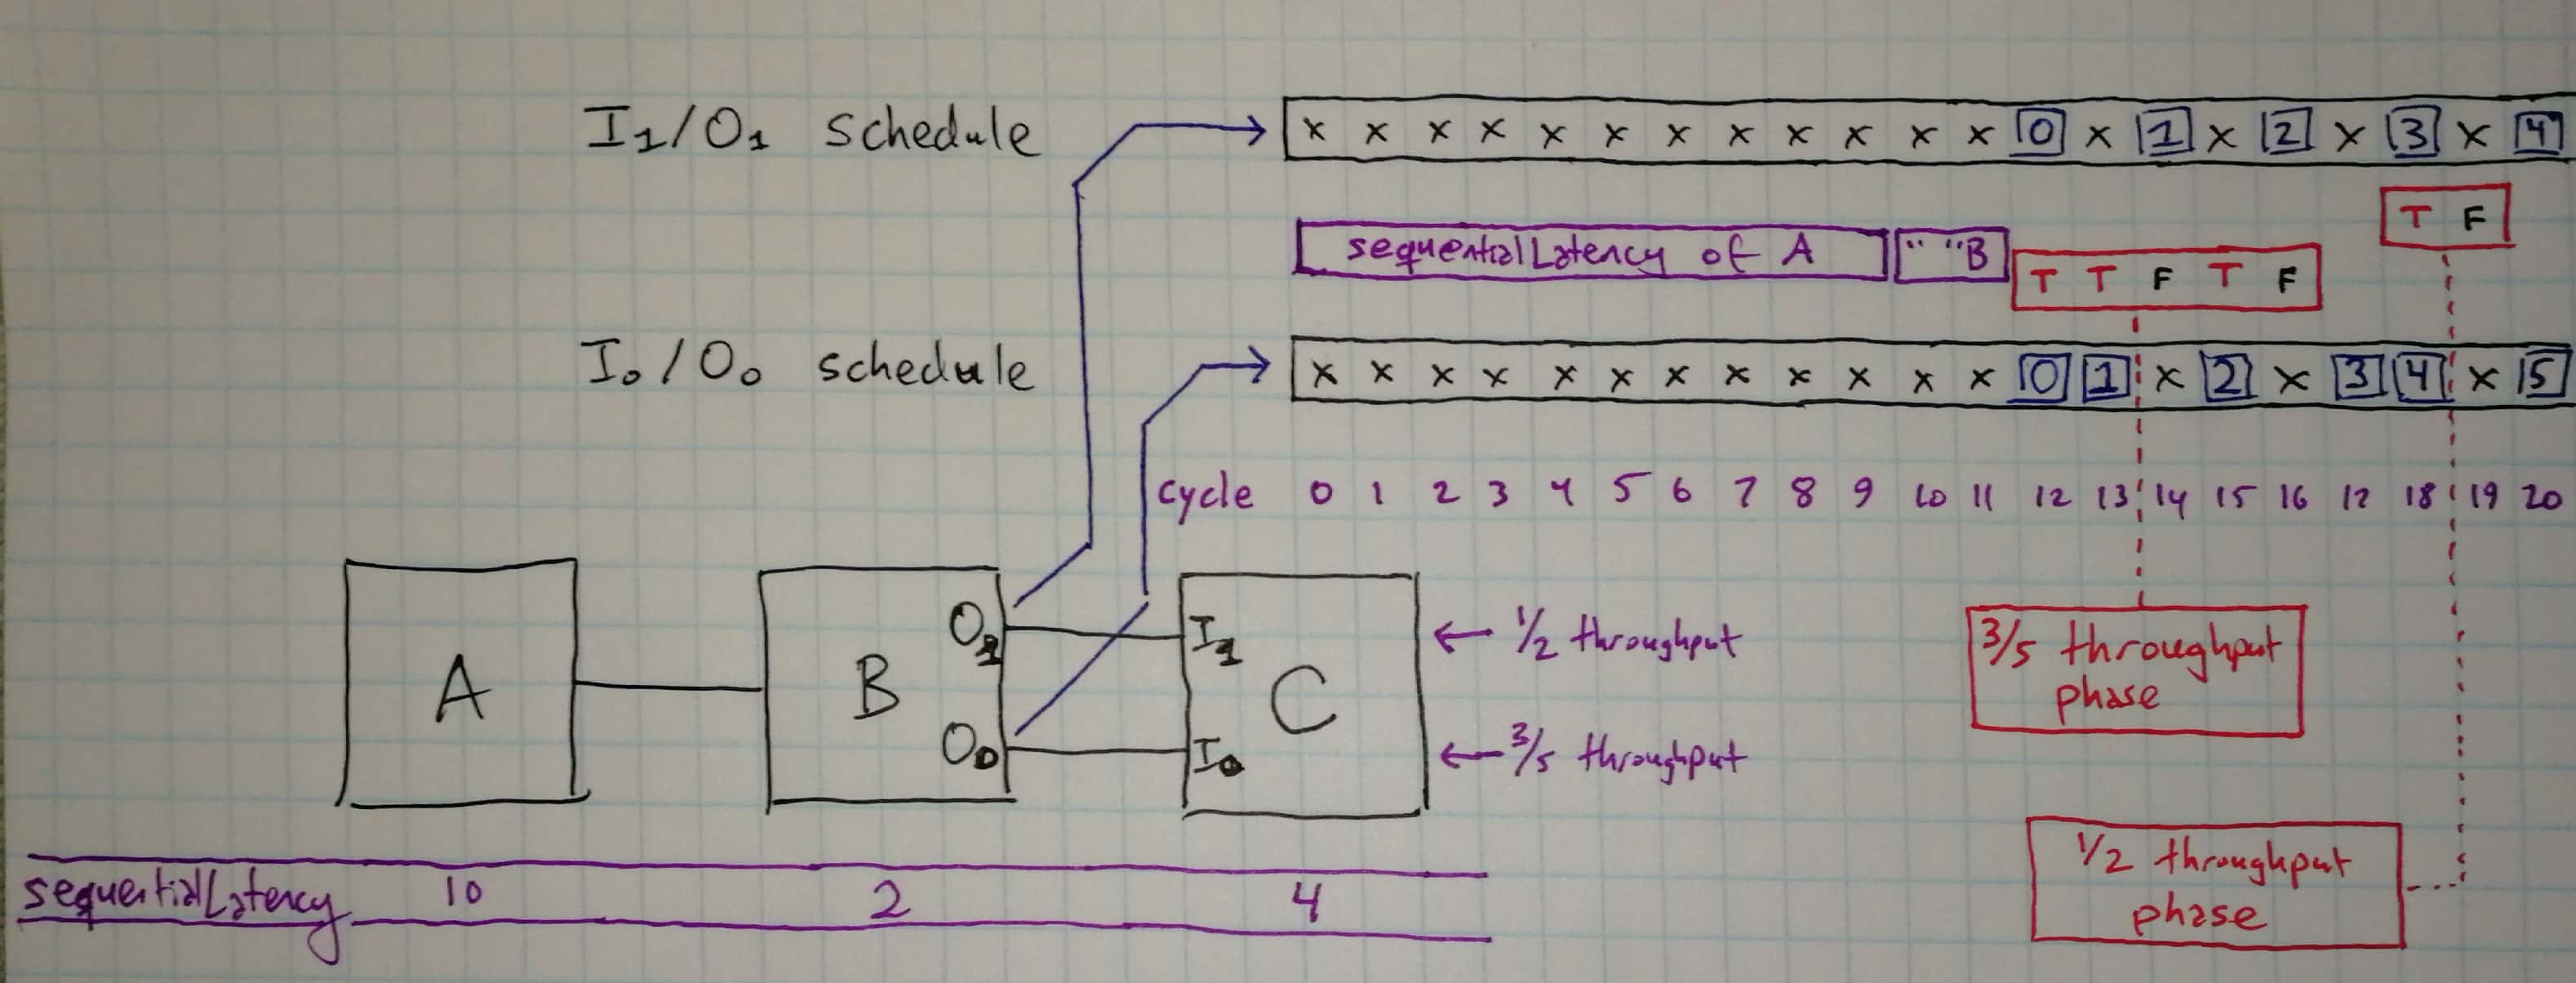
\includegraphics[width=1.0\linewidth]{Figures/phase.jpg}
Visualization of scheduling based on \texttt{sequentialLatency}
wait and repeating phase pattern.
\end{center}

Consider the output pattern of $O_0$. We'll start with 12 cycles of
garbage, since 12 is the sum of \texttt{A} and \texttt{B}'s
\texttt{sequentialLatency}s, then $O_0$ will create valid outputs on
cycles 12, 13, 15, 17, 18, 20, 22... (since the $\frac{3}{5}$ phase
indicates the $0^{th}, 1^{st},$ and $3^{rd}$ cycles in each 5-cycle
pattern is valid). Meanwhile, valid output will be sent through $O_1$
on cycles 12, 14, 16, 18, 20, 22...

This matches what \texttt{C}'s input ports $I_0$ and $I_1$
expect. They'll wait 12 cycles since 12 is the sum of the upstream
ops' \texttt{sequentialLatency}s, then, by looking up the same phase
pattern, \texttt{C} can reproduce the exact schedule that \texttt{B}
used. ($I_0$ expects input on cycles 12, 13, 15, 17...; $I_1$ on
cycles 12, 14, 16...).

Finally, note that the initial inputs and initial outputs are always
synchronized across ports. $O_0$ and $O_1$ start output on cycle 12,
and $I_0$ and $I_1$ start expecting input on cycle 12. This means that
the definition of \texttt{sequentialLatency} is well-defined. Using
the definition, we expect that each input port of \texttt{B} should
start accepting input on cycle 10, and each output port of \texttt{C}
should emit its first valid output on cycle 16.

\subsection{Phase Assignment Algorithm}

The throughput-to-phase assignment algorithm is based on the
\texttt{SequenceArrayRepack} op. This op converts between
sequences of arrays of different sizes. (In Aetherling terms, a
sequence is a stream of valid values delivered across multiple,
not-necessarily-contiguous clock cycles -- in the earlier
example, port $O_0$ delivers a 3-sequence of outputs on cycles
12, 13, and 15).

For example, a (fully utilized) \texttt{SequenceArrayRepack} that
converts from 1-sequences of 2-arrays to 2-sequences of 1-arrays would
take a valid 2-array input on cycles 0, 2, 4... and, using values
unpacked from the input arrays, generate a 1-array output on each
clock cycle.  On each even-numbered cycle, one entry of the input
2-array won't fit in the output 1-array, and will be ``leftover''
(i.e. buffered) for output on the next clock cycle.
% I wish that I just wrote ``buffered'' instead of ``leftover'' on
% all my hand-drawn charts. Oh well.

\begin{center}
% I'm so tired of figures ending up pages away and having to
% constantly fight with htb!!1! and friends so against all advice
% otherwise I'm ditching floating environments except when I
% personally feel like using one.
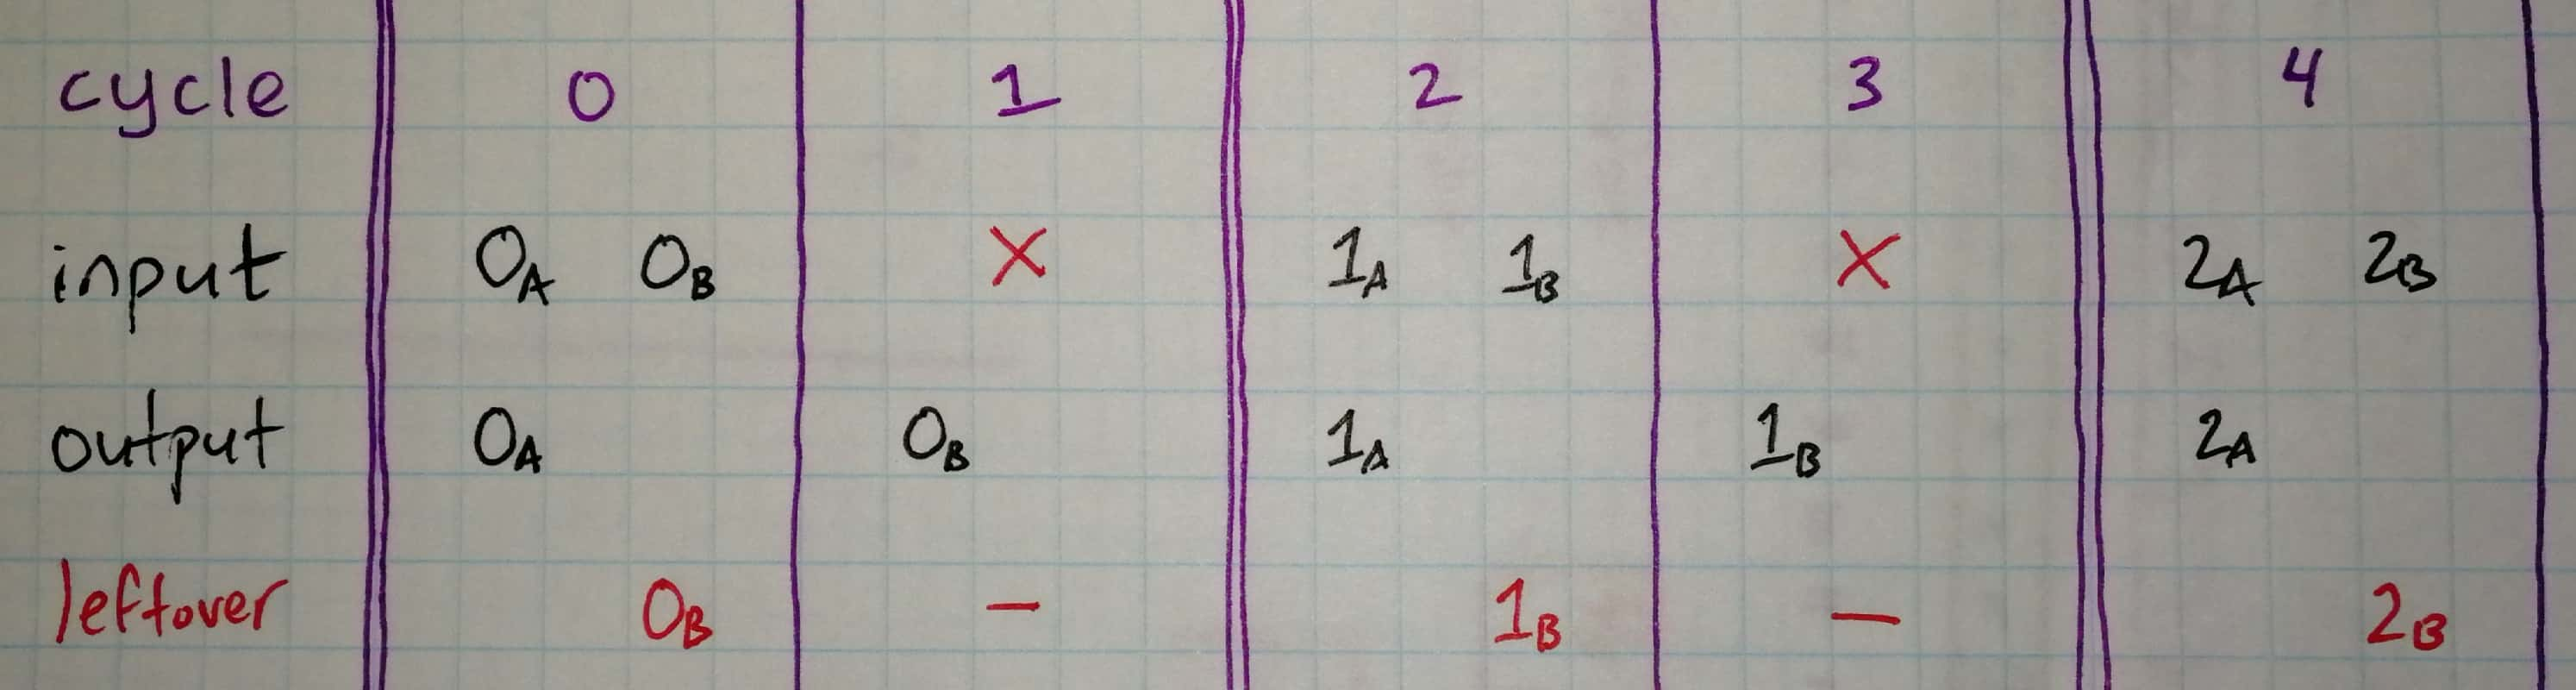
\includegraphics[width=1.0\linewidth]{Figures/repack.jpg}
\texttt{SequenceArrayRepack (1,2) (2,1)} repacking 2-arrays to 1-arrays.

Each sequence gets its own digit.
\end{center}

To determine the pattern for an $\frac{x}{Y}$ throughput, we figure
out what pattern would be most convenient for the input of a
fully-utilized \texttt{SequenceArrayRepack} converting $x$-sequences
of $Y$-arrays to $Y$-sequences of $x$-arrays. This is a ``narrowing''
repack: the output arrays are narrower than the input arrays since
\begin{equation*}
    \text{throughput}<1 \implies x<Y
\end{equation*}
The repack is fully utilized, so the output comes
out at maximum rate: $Y$ outputs over $Y$ clock cycles (in Aetherling
terms, output \texttt{seqLen=cps=Y}).

It would be most convenient for the \texttt{SequenceArrayRepack} if
each input array came in as soon as it was needed, but no sooner.
(This is convenient in the sense that it minimizes internal
buffering). Earlier, I set the $\frac{3}{5}$ throughput phase to
\texttt{[True, True, False, True, False]}. This pattern can be
reproduced by working through what a fully-utilized 3-sequence,
5-array to 5-sequence, 3-array \texttt{SequenceArrayRepack} input
schedule should be. Make a table with 5 columns, one for each clock
cycle 0-4 (fully-utilized $\implies$ \texttt{cps=5}), and have entries
for inputs, outputs, and leftovers in each column.

\begin{center}
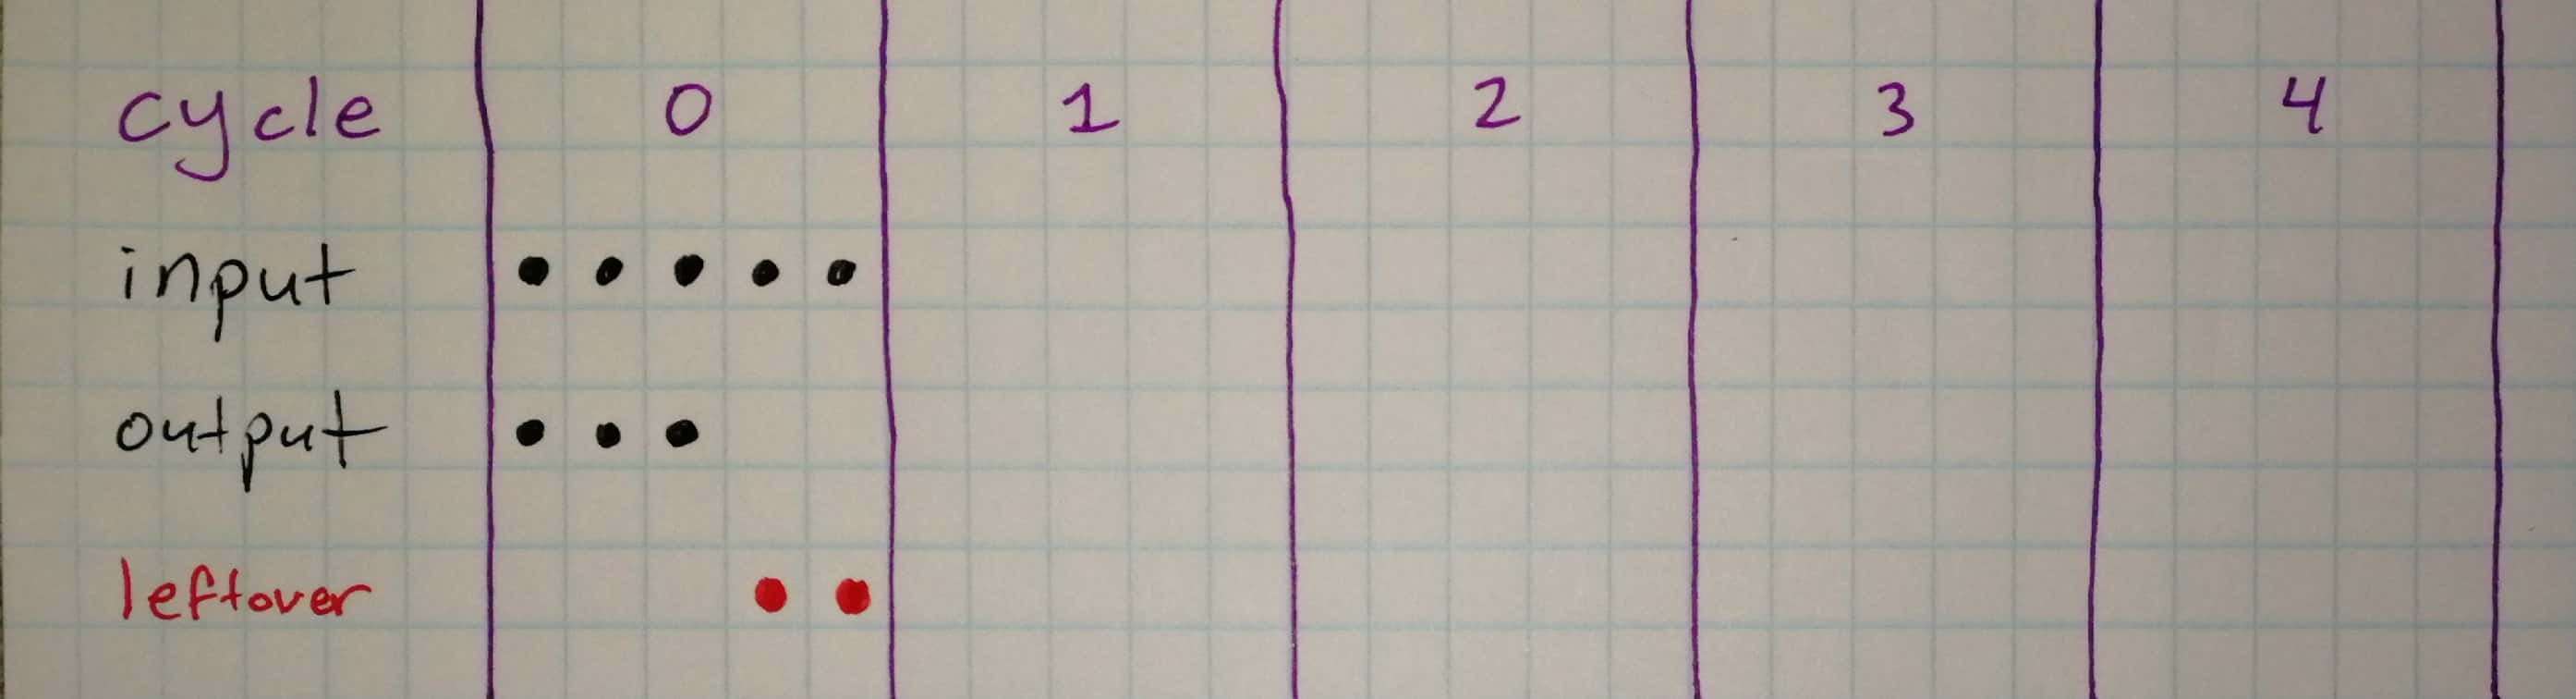
\includegraphics[width=1.0\linewidth]{Figures/sorry-if-patronizing.jpg}
Visual aid. Fill in the chart for the next example.

\texttt{SequenceArrayRepack (3,5) (5,3)}
\end{center}

On each clock cycle, one 3-array output must be produced. Represent
this by drawing 3 dots in the output cells. This $0^{th}$ cycle's
output must come from some input, so one 5-array input must come in
on the $0^{th}$ cycle, leaving 2 array entries left over that must
be stored in \texttt{SequenceArrayRepack}'s internal buffer. Draw
5 dots in the $0^{th}$ input cell and 2 dots in the $0^{th}$
leftover cell to represent this.

2 array entries alone are not enough to populate the $1^{st}$ cycle's
3-array output, so on that cycle we must read in another 5-array
input. By cycle 1 then, the repack will have read in 10 and output 6
array entries, leaving 4 stored internally. Draw 5, 3, and 4 dots in
the first column to represent this (input, output, leftover).

Now that there's 4 array entries buffered, we can produce another
3-array output on the $2^{nd}$ cycle without reading in another array.
By the earlier rule, we defer reading in another valid input for now,
producing the 3-array output using buffered inputs. Fill in 3 output
dots and 1 leftover dots in column 2 to represent this.

Fill in the last 2 columns using the same rule. There should be
input 5-arrays on cycles 0, 1, and 3, leading to the phase pattern
\texttt{[True, True, False, True, False]}. For each cycle 0-4, there
should be 2, 4, 1, 3, and finally 0 leftover entries.\footnote{
That there are 0 leftover entries at the end is notable: we would
just repeat if we continued the phase pattern for another 5 cycles.
If the throughput fraction $\frac{x}{Y}$ were not in reduced form, we
would still get the same phase (recall that phase repeats, so
\texttt{[True, False]}-repeated $\equiv$ \texttt{[True, False, True, False]}-%
repeated. Although I've explained this as a fraction-to-phase mapping,
in practice it's a mapping of \texttt{seqLen}$\equiv x$ and
\texttt{cps}$\equiv Y$ to phase, so it's not actually guaranteed
\textit{a priori} that two ops with matching fractional throughputs
will have matching phase if the $\frac{\text{seqLen}}{\text{cps}}$
fractions aren't in reduced form. That the phase is still the same
without reduced fractions is pretty important to this scheme, but
no one else seemed to be worried about this so it's in this footnote
here.

Actually, there's one last thing to note, which is that an
X-array to Y-array \texttt{SequenceArrayRepack} has the same schedule
(all else being equal) as an nX-array to nY-array repack, $n:$integer.
This is the other half of the phase being the same without reducing
fractions.

If you think about the dot chart from earlier, each input, output,
and leftover cell will have a multiple-of-$n$ number of dots. The
chart would be equivalent if we represented each group of $n$ dots
as a single dot, matching the original X-array to Y-array repack's chart,
and therefore its schedule.}
% I just had to point all that out.

\subsection{SequenceArrayRepack Example}

I propose that all ops conform to this phase scheme, including
\texttt{SequenceArrayRepack} itself. It's a bit hard to explain my
proposed \texttt{SequenceArrayRepack}'s behavior because of pontential
confusion between the concrete \texttt{SequenceArrayRepack} being
analyzed and the imaginary \texttt{SequenceArrayRepack}s used to
determine phase patterns.

Let's work through the behavior of a repack that accepts as input
4-sequences of 3-arrays, produces 3-sequences of 4-arrays, and has
\texttt{cps=}6. This repack has an input throughput of
$\frac{4}{6} = \frac{2}{3}$
and an output throughput of $\frac{3}{6} = \frac{1}{2}$.\footnote{
As explained in another footnote it doesn't really matter if these
fractions are reduced, but it makes the example cleaner.
}

Determining the input and output phases requires us to construct a
couple of \texttt{SequenceArrayRepack}s that don't really resemble the
repack we're analyzing -- analyzing their input schedule as we did
above, we'll get an input phase of \texttt{[True, True, False]} and an
output phase of \texttt{[True, False]}. Focusing back on the original
\texttt{SequenceArrayRepack} we're analyzing, if we just repeat this
phase pattern without any added latency, some array entries will be
scheduled for output before they were scheduled for input, so we need
to have \texttt{sequentialLatency=1}.

\begin{center}
% I'm a minus-sign girl in a camelCase world.
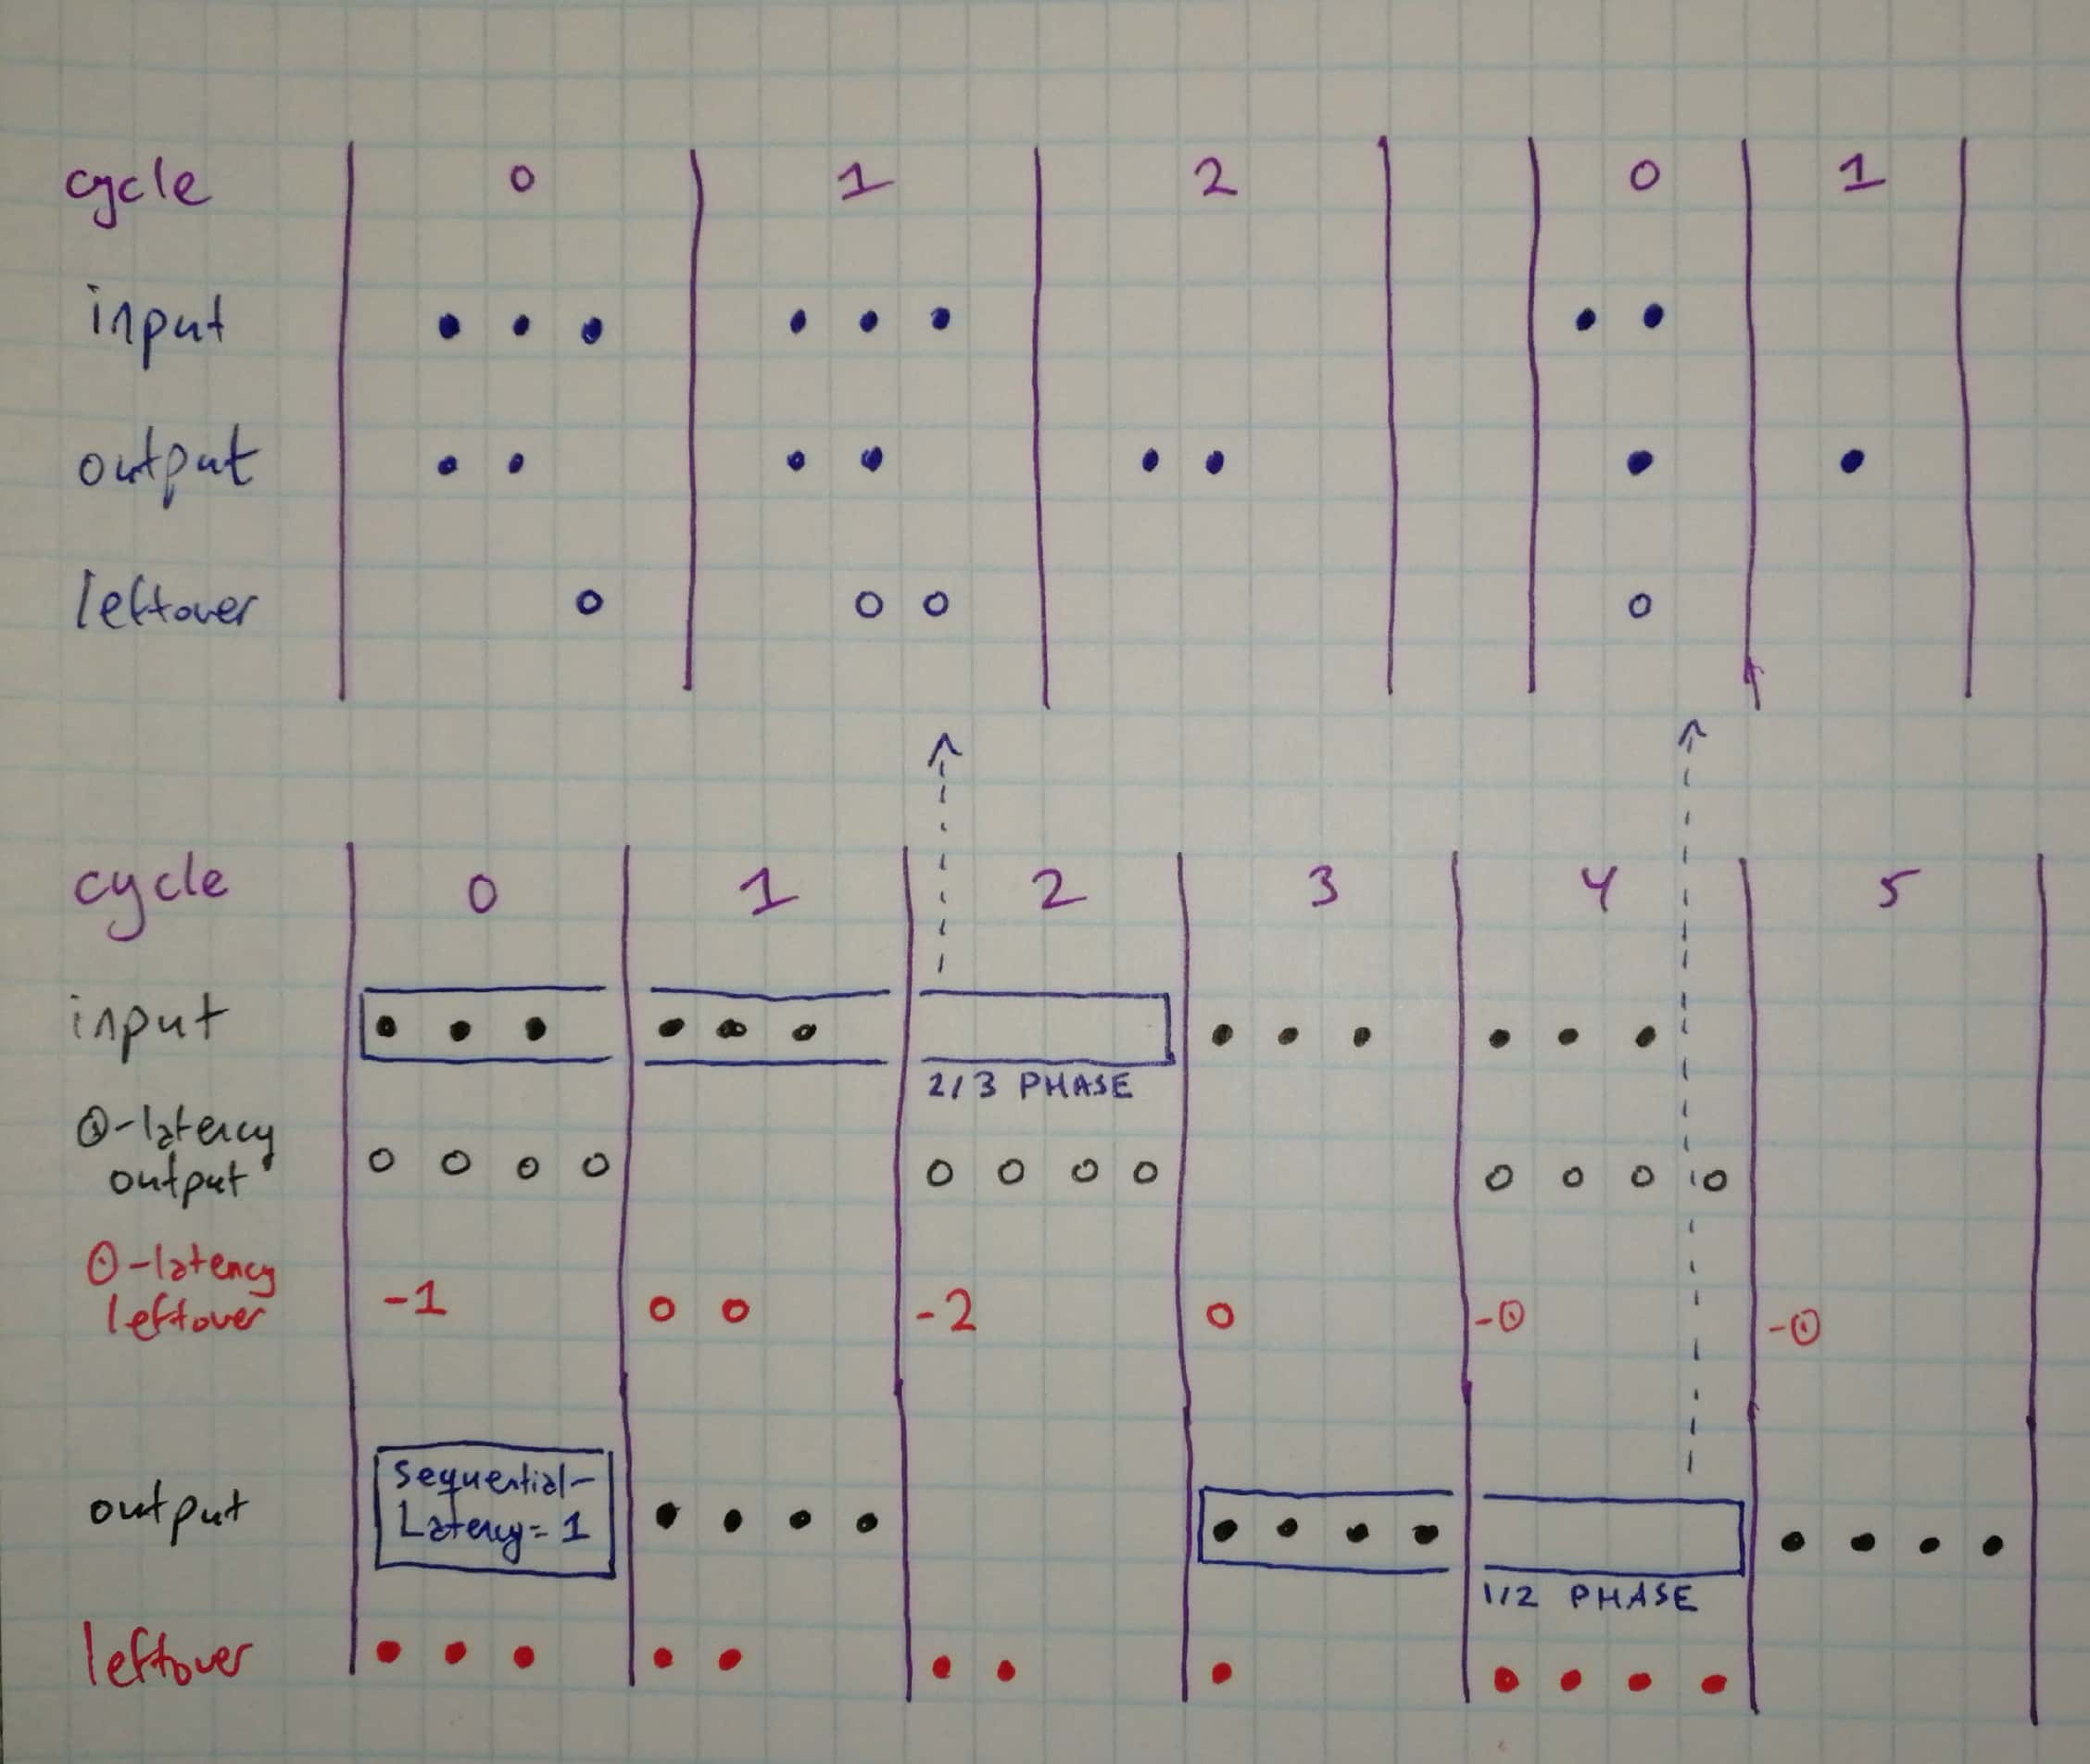
\includegraphics[width=1.0\linewidth]{Figures/underutil-repack.jpg}
Example of underutilized 3-sequence of 4-array to 4-sequence of
3-array \texttt{SequenceArrayRepack} (\texttt{cps=6}). The bottom
chart shows the schedule of the actual repack being analyzed (negative
entries on the 0-latency leftover row illustrate the problem of array
entries travelling backwards in time without added latency). The top
two charts represent the imaginary line buffers used to determine the
input and output phase.
\end{center}

\newpage
As another example, consider the widening counterpart of the first
line buffer example. This widening line buffer converts from
5-sequences of 3-arrays to 3-sequences of 5-arrays, with
\texttt{cps=5}. (Figure \ref{widening.jpg})

\begin{figure}[bth]
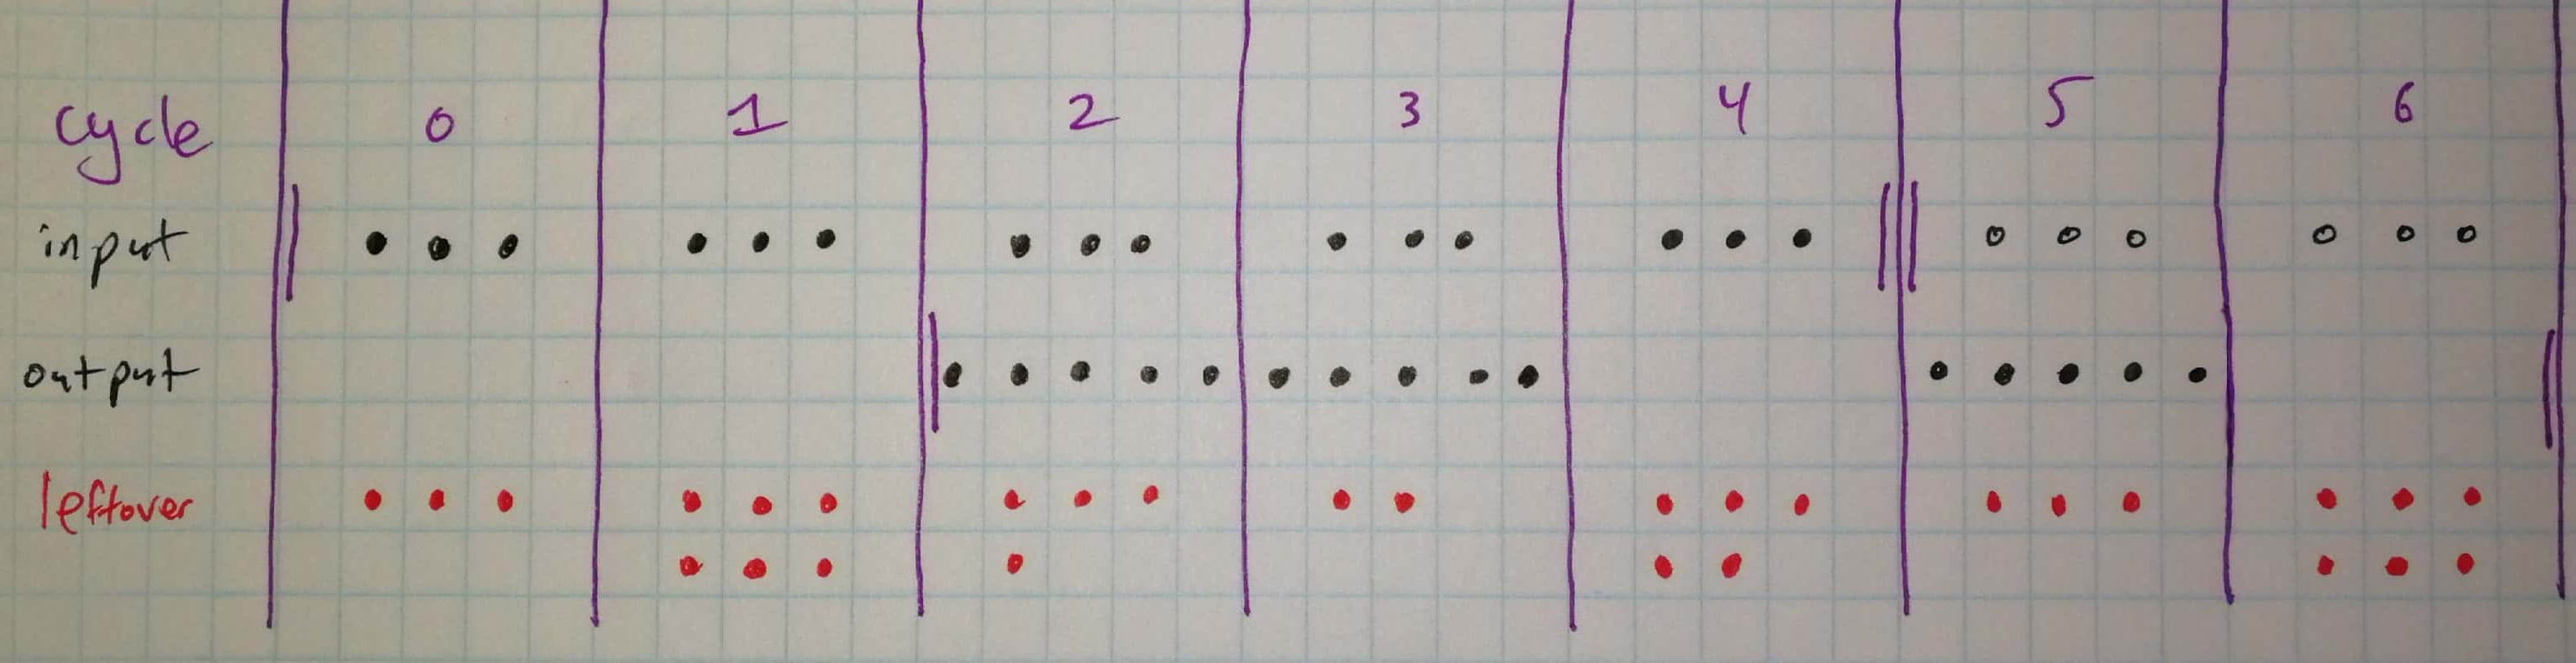
\includegraphics[width=1.0\linewidth]{Figures/widening.jpg}
Widening repack schedule (\texttt{SequenceArrayRepack (5,3) (3,5)}).

\caption{\texttt{sequentialLatency=2}; the initial valid output comes 2 cycles
after the initial valid input.}
\label{widening.jpg}
\end{figure}

Here, the input phase is \texttt{[True]} based on input throughput 1,
and the output phase is \texttt{[True, True, False, True, False]}
based on looking up the phase for output throughput
$\frac{3}{5}$. This phase matches what the corresponding narrowing
repack (\texttt{SequenceArrayRepack (3,5) (5,3)}) expects -- indeed,
under this plan, this widening repack can have its schedule matched
with any other op with throughput $\frac{3}{5}$.

\subsection{Rationale \& Alternatives}

The issue with requiring a consistent phase pattern across ops is that
an op may be forced to have more latency (and therefore more buffer
space needed) than theoretically required. For
\texttt{SequenceArrayRepack (3,5) (5,3)}, (Figure \ref{widening.jpg})
the \texttt{sequentialLatency} cannot be decreased to 1 with this
output phase (we'd have negative leftover inputs at cycle 2). With
\texttt{sequentialLatency=2}, the widening repack always has at least
one value buffered on each clock cycle, and, on cycles 1,4,6... will
have a full output array's worth of leftover outputs.  In principle
latency and buffering could be reduced by emitting arrays at cycles 1,
3, and 4 instead of 2, 3, and 5, adopting the alternate phase
\begin{equation}
    \texttt{[True, False, True, True, False]} % Double check
    \label{alternate-phase}
\end{equation}

\begin{center}
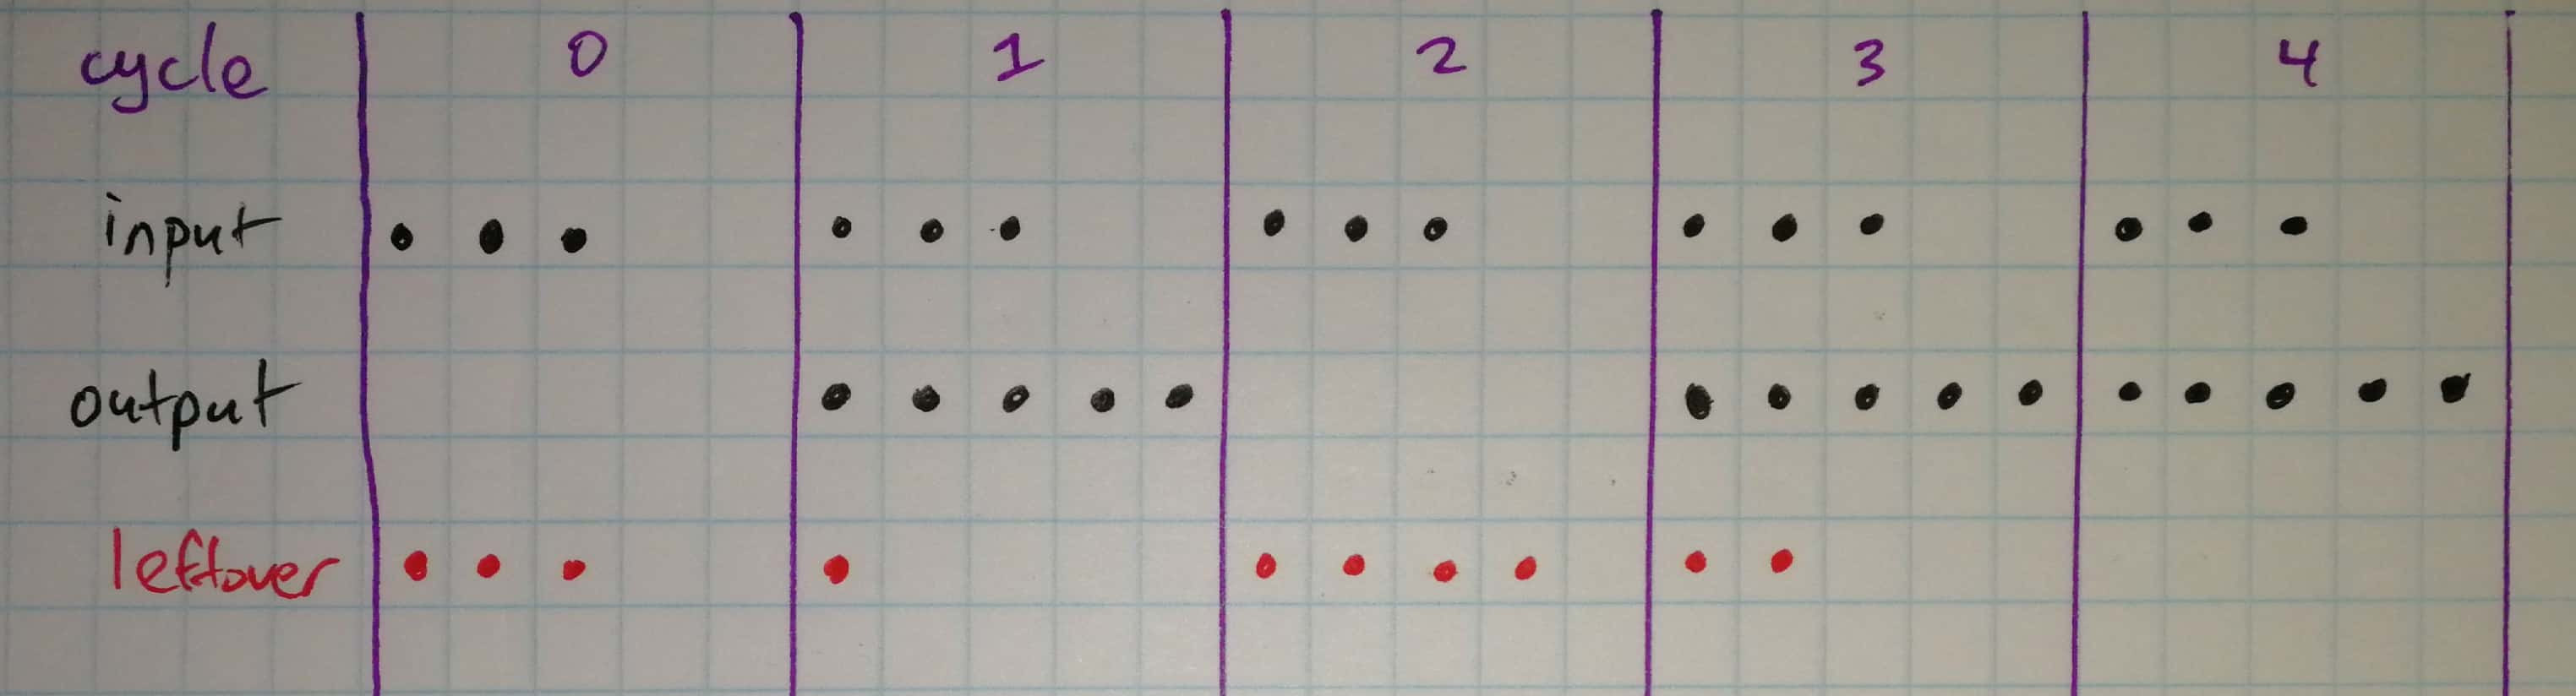
\includegraphics[width=1.0\linewidth]{Figures/alternate-widening.jpg}
\end{center}

The problem with not matching phase is that, while translating Haskell
IR to actual hardware, we'll have to add additional phase-matching
buffers between ops with matching latencies but different phase
patterns.

As an example, consider two options for wiring a widening repack to
its corresponding narrowing repack.\footnote{This is a contrived
  example, but the costs illustrated also apply to more realistic
  circuits where there is logic inserted between the two
  \texttt{SequenceArrayRepack}s.  } Option A is for the widening
repack to adopt the phase that the narrowing repack expects (as I
propose). Option B is for the widening repack to adopt the alternate
output phase at (\ref{alternate-phase}), and for a phase-matching
device to be placed between the two repack ops.

\begin{center}
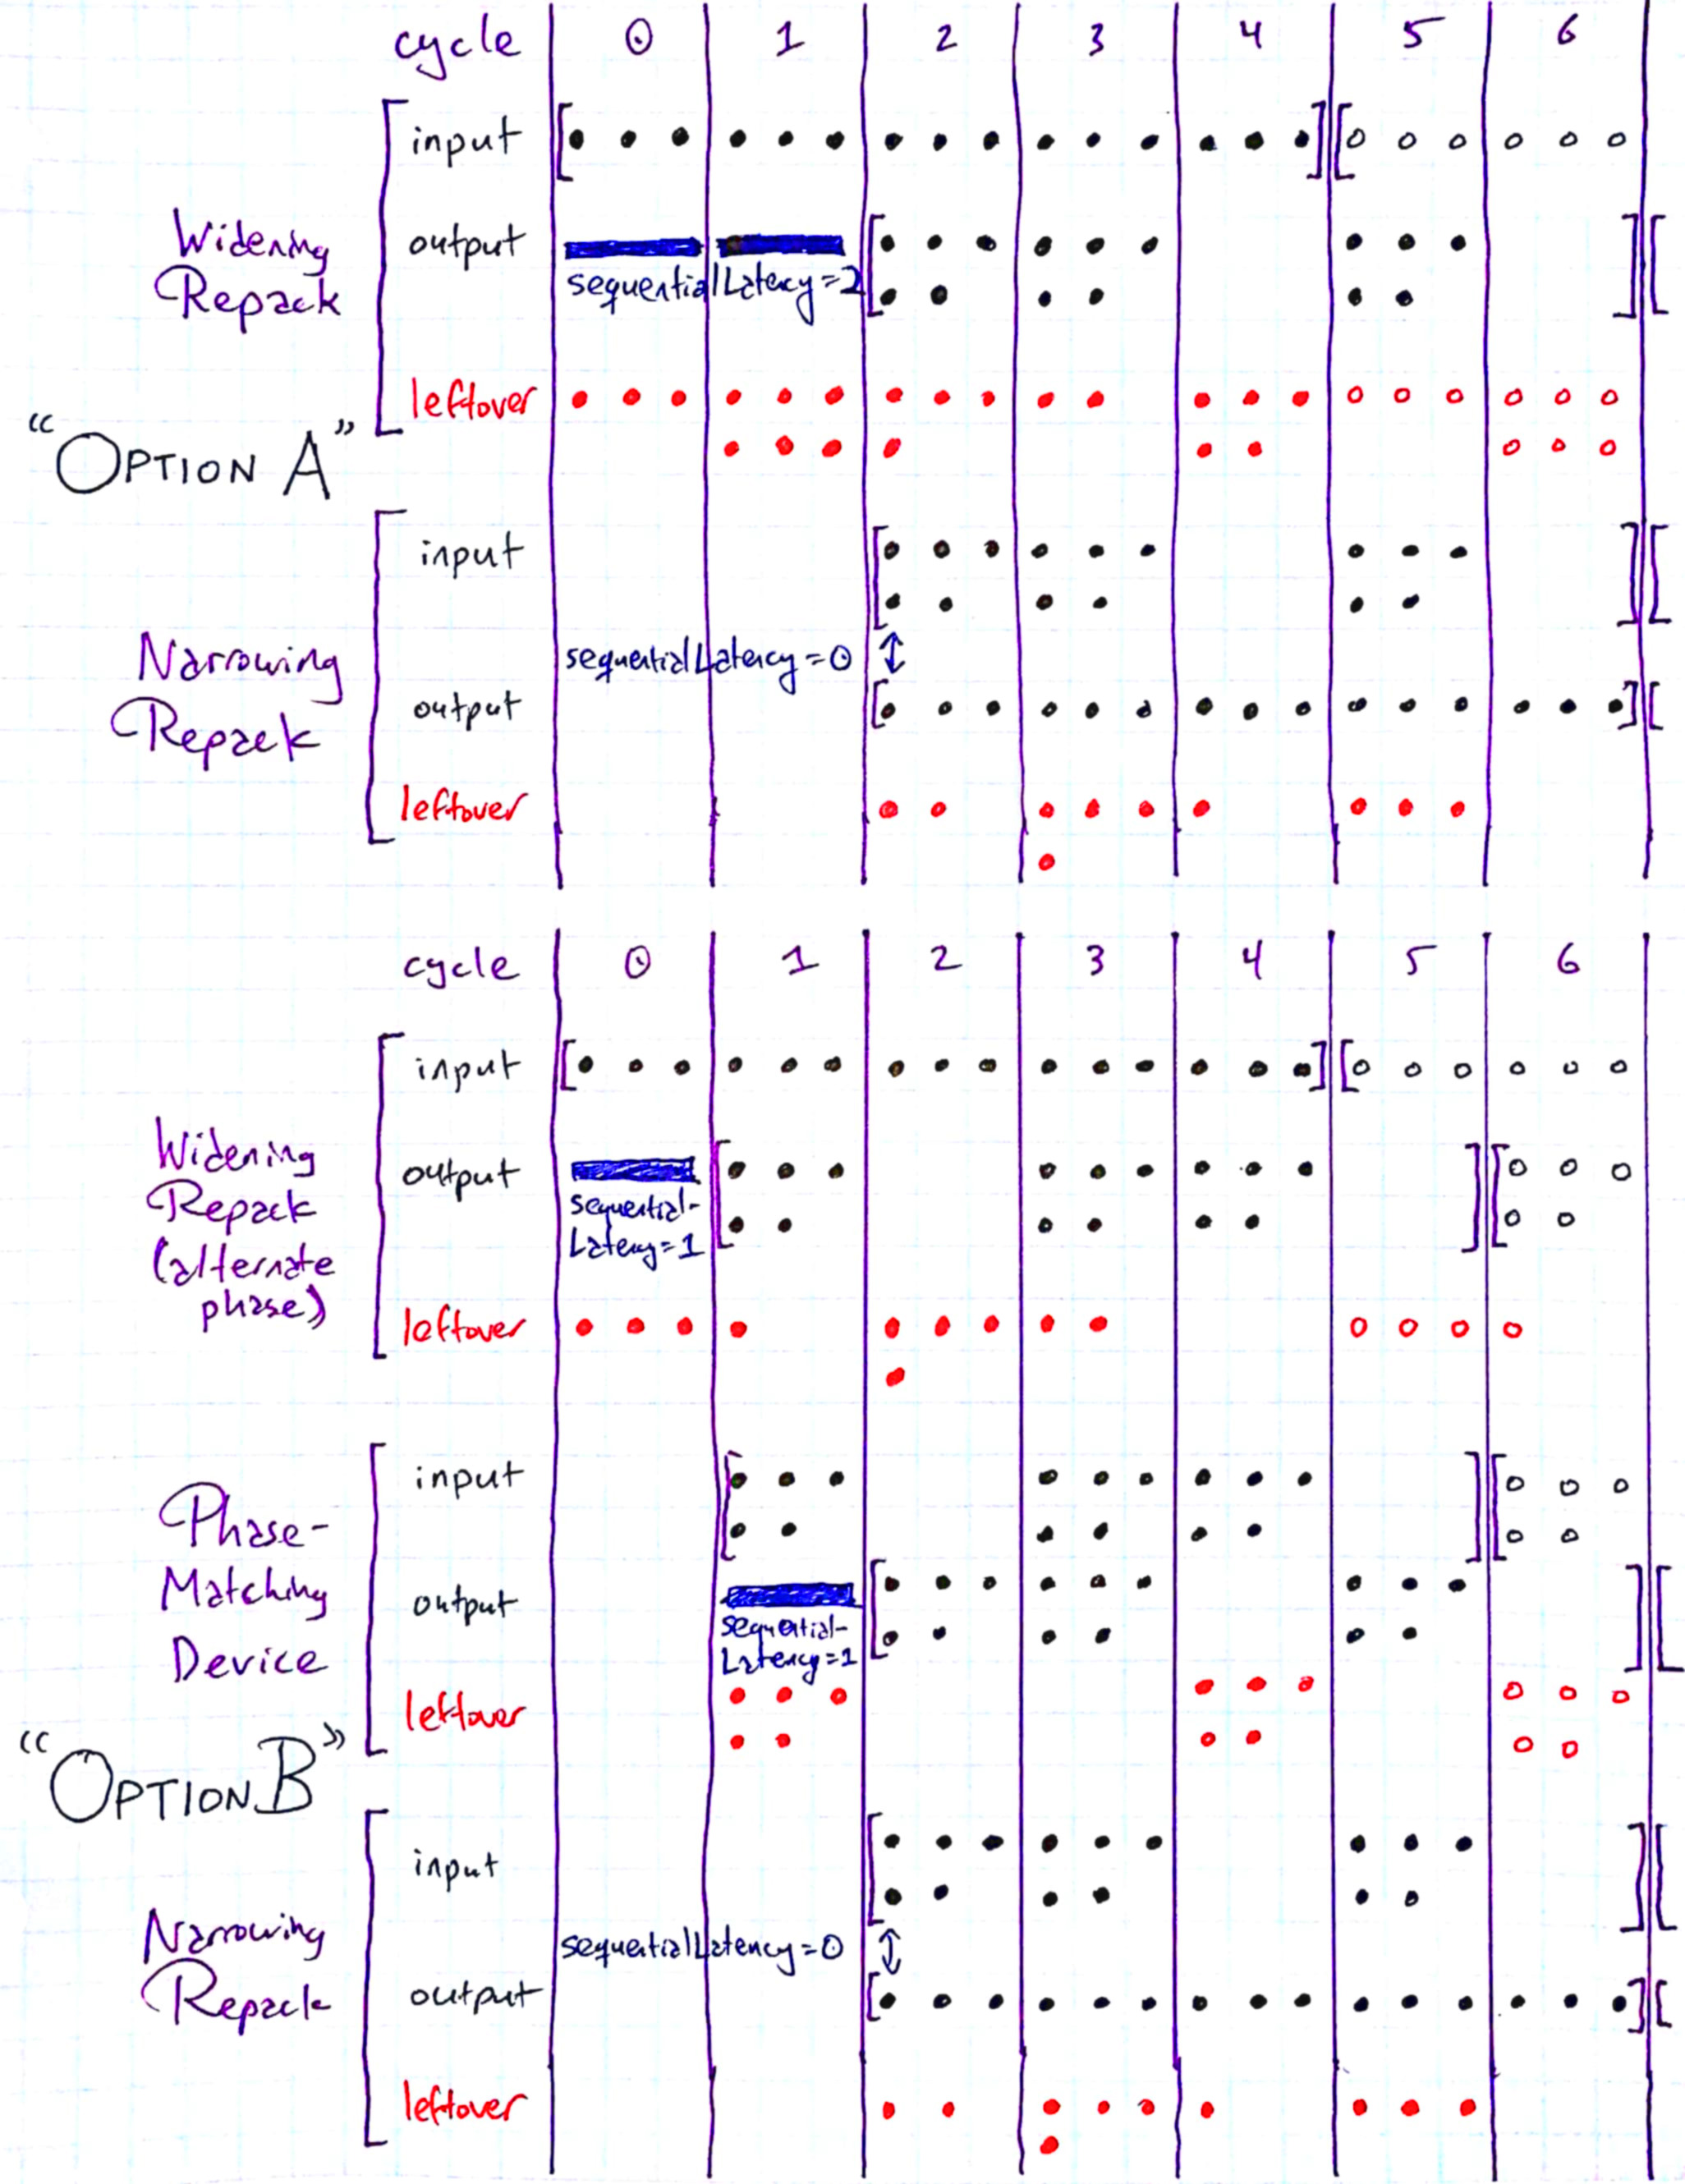
\includegraphics[width=1.0\linewidth]{Figures/phase-comparison.jpg}
Comparison of two options: top is my proposal, botton is rejected alternative.

Information flows from top-to-bottom.
\end{center}

First, at least in this example, the latency decrease of the alternate
widening \texttt{SequenceArrayRepack (5,3) (3,5)} is cancelled out by
the 1 latency increase introduced by the phase matching device.  I
suspect that any circuit area decrease by reducing buffer space in the
widening repack would also be cancelled out by the buffers in the
phase matching device. In fact, the area of option B is probably
higher that option A, because the phase matching device would need its
own duplicate of the muxes and counters that the repack devices
presumably use in their implementation. Think of it this way:
conceptually, the widening repack in option A combines the
functionality of the phase-matching device and widening repack in
option B, using only one counter and set of muxes to do so.

In my view though, the major issue with automatically adding
phase-matching devices is that this adds extra cost and latency not
visible in the Haskell IR, which
\begin{enumerate}
\item makes it more difficult for the user to reason about the latency
and area of a circuit represented in Haskell IR form.

\item makes my \texttt{ComposePar} retiming passes less useful (or much
more difficult to write), with the true latency of different paths of
the circuit impossible to compute from the Haskell IR alone, which does
not provide phase information.
\end{enumerate}

Another alternative I considered and rejected was a simpler
throughput-to-phase mapping (or at least a mapping simpler to
explain). The phase pattern for a $\frac{x}{Y}$ throughput could have
just been $x$ valid values followed by $Y-x$ garbage values.
The issues with this approach are:
\begin{enumerate}
\item This would increase the buffer space needed in a
  \texttt{SequenceArrayRepack} (which is ultimately the source of
  fractional underutilization). Intuitively, even for widening repacks
  and underutilized repacks, for which my proposed phase would not be
  the one that is theoretically most efficient, it would still be more
  expensive to have all inputs or outputs scheduled at the start or
  end of a pattern rather than spread out through time, as my proposed
  phases require.

\item Using this mapping, we could only assume that two ports with the
  same throughput will have matched phases if the throughput fraction
  $\frac{x}{Y}$ is always in reduced form. The actual
  throughput-to-phase mapping I propose does not require fractions to
  be in reduced form; for non-reduced fractions $\frac{nx}{nY}$ my
  proposed mapping naturally creates a phase that just repeats itself
  $n$ times. This seemed more elegant to me than manually reducing
  fractions.\footnote{In hindsight this isn't all that great a reason
    (the buffer space reason is more practical), but I include it
    because this is probably the real reason I prefer the more
    complicated-to-explain throughput-to-phase mapping I proposed.}
\end{enumerate}

% The widening repack is a bit more expensive than it needs to be.
% With alternate output phase, can have sequentialLatency=1.
% If we don't standardize phase, some ops may be more efficient in
% isolation, but when we wire them together we'll need some
% buffers that match up phase. This adds invisible cost and latency.
% Imagine wiring up the alternate repack and original narrowing repack.

\section{Test Writing}

The tests I designed include
\begin{enumerate}
\item

Haskell tests for the functional simulator I designed.

\item

Python tests for the hardware line buffer David Durst is
implementing in Magma based on ``The Line Buffer Manifesto''
specifications. These tests use the CoreIR simulator.

\item

Tests for the sequential compose (\texttt{|>>=|}) and parallel
compose (\texttt{|\&|}) Haskell Aetherling operators. These tests
check that the produced Haskell IR node is correct given valid
operands, and check that the operators reject invalid operands
(mismatched port types, mismatched synchronous and ready-valid
timing, and mismatched throughputs with synchronous timing).

\item Tests for the \texttt{ComposePar} retiming passes. There are
$18+$ test cases, some of which have compose ops nested several
layers deep meant to check for corner cases.
\end{enumerate}

\end{document}

